\nwfilename{appendices.nw}\nwbegindocs{0}\newpage% ===> this file was generated automatically by noweave --- better not edit it

\begin{appendices}
%\renewcommand{\thesection}{\Roman{section}\;\;}
\renewcommand{\thesection}{\Alph{section}}

\section{Installing and running the Code}
\label{sec:install}

The program can be downloaded from Github: \url{https://github.com/gtelang/tspnng}. Alternatively
open a terminal and run the command, \texttt{git clone https://github.com/gtelang/tspnng.git}

The only other prerequisites for running the code, are the 
\href{https://www.anaconda.com/products/individual}{Anaconda} distribution of Python 3 
and a couple of other packages.  To check if the Python executable is in your path \footnote{and that it is Python 3.7 or above}
run the command \verb|python --version|. If it succeeds, you have installed Anaconda! 

The additional packages required can be installed by: 

\begin{quote}
\color{blue}
\texttt{pip install colorama prettytable tsp satispy treelib} \footnote{If you don't have superuser access during installation or the installation process seems to get stuck, add the flag \texttt{\color{red} \texttt{-{}-}user} at the end}   \\
\texttt{git clone https://github.com/jvkersch/pyconcorde} \\
\texttt{cd pyconcorde}\\
\texttt{pip install -e .}
\end{quote}

%#If the installation of \texttt{pyconcorde} fails, that's okay!; the code will switch to the much slower Python based TSP solver that also computes optimal solutions. 
%This slower package can compute tours of size upto 30 to 40 in a few seconds; lareger point-clouds will take more than a couple of minutes.  

To run the program, \texttt{cd} into the code's top-level folder, then type \footnote{On Windows replace, the forward slash `/` by `\textbackslash`}
any one of (depending on your use case): 

\definecolor{alizarin}{rgb}{0.82, 0.1, 0.26}

{\LARGE \color{alizarin}
\begin{itemize}
\item \texttt{python src/main.py \textit{-}\textit{-}interactive}
\item \texttt{python src/main.py \textit{-}\textit{-}file \textit{<filename>}} 
\item \texttt{python src/main.py \textit{-}\textit{-}tsplibinstance \textit{<instancename>}}
\end{itemize}
}

The `\textit{-}\textit{-}interactive` flag is for inserting a 
point-set with the mouse onto the canvas. 

The `\textit{-}\textit{-}file \textit{<filename>}' is for inserting a 
custom point set provided in a file onto the canvas  (and if needed 
modifying the point set by adding more points). 

When entering input points with a file make sure the file looks similar 
to the contents of the \verb|foo.yaml| in the home directory of the code 
whose contents I've also shown in \autoref{fig:fooyaml}. Make sure that 
all coordinates are scaled so that the points in the file lie inside the unit-square. This makes it convenient 
for nice plotting and for different experiments. 

Finally, very much similar to the last option but only for TSPLIB instances, we have
`\textit{-}\textit{-}tsplibinstance \textit{<instancename>}' where you just enter the filename
corresponding to the appropriate TSPLIB instance. For instance by typing
`python src/main.py \textit{-}\textit{-}tsplibinstance berlin52' runs the code 
on the `berlin52' instance of TSPLIB. 

\begin{mdframed}
{\color{alizarin} 
The code takes care of retrieving the appropriate file corresponding to each instance. Do not 
type `.yml' extension or directory name or anything like that when entering in the instance name. e.g. see how the `berlin52'
instance was passed to the code in the previous sentence}
\end{mdframed}

The list of instance names and the corresponding pictures can be found in can be found in Appendix \autoref{sec:catalog}. 

\begin{figure}[H]
  \centering
  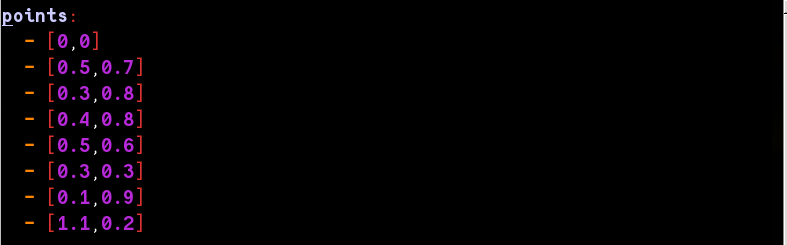
\includegraphics[width=12cm]{miscimages/fooyaml-screenshot.png}
  \caption{\label{fig:fooyaml} Contents of the sample \texttt{foo.yaml} file in the home directory for inputting custom points into the code}
\end{figure}




\begin{mdframed}[backgroundcolor=black!10,rightline=false,leftline=false]
\textbf{UPDATE}: (\textit{Thanks Logan!!}) Some of you \textit{might} face problems running the code if you work with the newest Anaconda distribution
of Python 3.8.6, rather than Python 3.7.3 which I use. 

If you face this issue, please look at the screenshot \autoref{fig:loganinstall} of Logan's email to fix the problem. 
I leave my installation instructions above unchanged, in the event it works for some of you, so that you don't have to bother
mucking about with code-internals. 

In any event, Logan's suggested fix, is simple enough. 
   
\begin{figure}[H]
  \centering
  \fbox{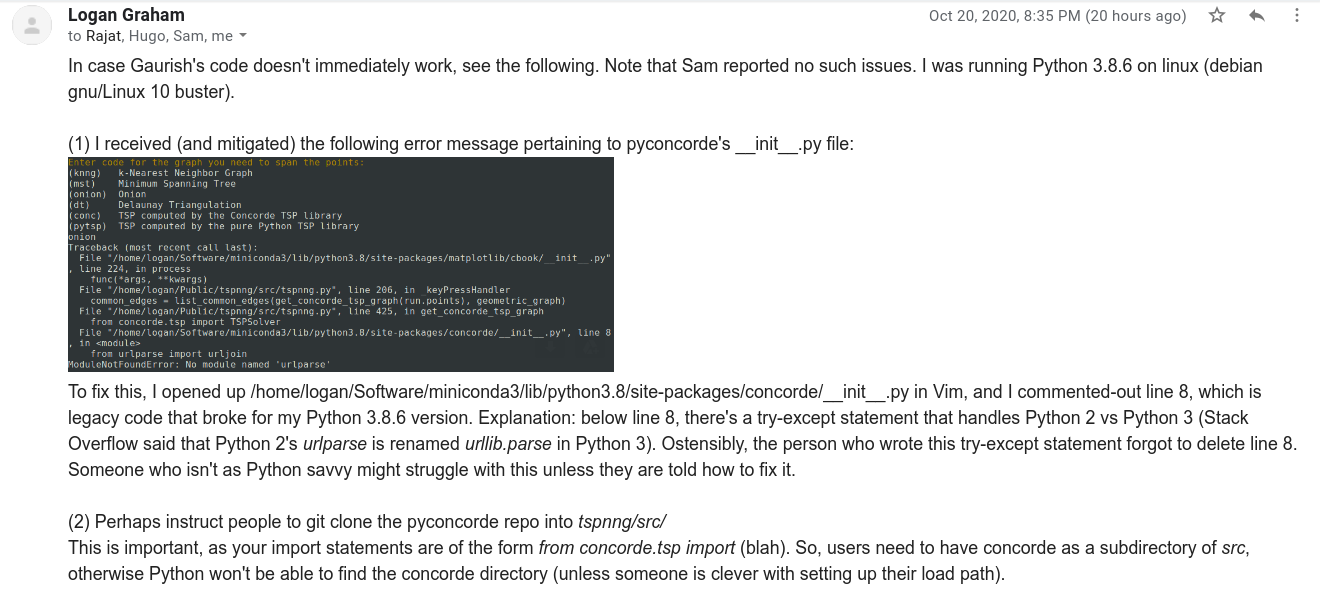
\includegraphics[width=16cm]{./miscimages/logan.png}}
  \caption{\label{fig:loganinstall} Screenshot of Logan's email with an installation fix}
\end{figure}
\end{mdframed}



As mentioned before one can mouse-in points onto a canvas (with double-clicks), or provide points via a file (and then add additional points via a canvas), 
run various network algorithms and render them onto a GUI canvas. \textit{\footnotesize By the way, make sure the terminal is visible at all times during your 
interaction with the canvas, as it will often ask for input via prompts or display output information.}


\begin{description}
\item[Entering points with mouse clicks] After you  mouse in your input points, press \colredt{i}; that will open a prompt at the terminal, asking which 
network do  you want computed on those points. Enter the code inside the brackets \colredt{(...)} 

\item[Generating large random point-sets on the canvas] If you \textit{don't} want to mouse-in points, and just need random points plastered uniformly across the canvas, 
press \colredt{u}, and then type into the terminal the number of points. Other kinds of non-uniform point sets can also be generated using the following 
     commands. 

     \begin{mdframed}
     \textit{Note that while computing these point-sets, if there are points ``left-over'', then the remaining points are added randomly and uniformly to the unit-square. }
     \end{mdframed}

     \begin{description}
         \item[Non uniform points] \textit{(This is kind of badly named, sorry, couldn't think of a better one \smiley} This a scheme I sometimes use when geneating non-uniform random points. Press \colredt{n} It generates clusters of points, wherein the clusters near the square boundary are ``tighter'' i.e. have smaller diameter.
         \item[Multi-modal distribution] Another scheme for non-uniform random points, that's more natural than the above one.  Press \colredt{m} and then type into the terminal the number of points, the number of modes, and the spread ($\sigma$)
              around each of the modes. The points are assumed normally distributed around each mode
         \item[Concentric circular points] Press \colredt{o} and then type into the terminal number of points and number of rings. 
         \item[Grid points] Press \colredt{g} and then type into the terminal, the number of points and then the number of rows of the grid. The number of columns
          is automatically computed. 
     \end{description}

\begin{mdframed}
  \textit{Note that after generating these points, you can continue mousing in additional points as part of the input. Useful 
  if you want, say, an example with more or less uniform randomly generated points, except for a few small tight clusters here and there. }
\end{mdframed}

\item[Computing TSP directly] \footnote{This is an option meant more for convenience than anything really; might be useful for trying to detect counter-examples}.   
To directly compute the TSP cycle on the points (without needing to go through the prompts of the previous step) just press \colredt{t}. 

\item[Canvas should be active during keypresses] Note that when you press, any of the keys above, your matplotlib canvas \textit{must} be an active window 
\footnote{Single click or tap the window title bar with the mouse to make the canvas active.} . Only \textit{then} 
does matplotlib detect the key presses (i.e. execute the appropriate call-back function).  

\item[Modifying input] If you want to insert another point onto the existing point-set, just double-click at that position on the canvas. 
The computed networks are wiped clean off the canvas, and you can again compoute the appropriate networks again as above. 

\item[Wiping the canvas clean] If you want the screen and the internal state wiped clean completely --- say, to begin tinkering with a fresh set of points --- press \colredt{c}. 
\end{description}

\vspace{2cm}


\begin{mdframed}
{\footnotesize \it
P.S: You may see a warning --- as I do --- in the terminal during key-presses:

\begin{quote}
\color{blue}
\texttt{CoreApplication::exec: The event loop is already running}
\end{quote}

{\color{red} Please ignore it!} It doesn't affect any of the results. Something in the
the internals of Matplotlib using Qt triggers that message. \shrug. 
If you have any trouble --- or detect a bug! ---  we can hash things out on Slack, Github or email.
}
}
\end{mdframed}







\section{Catalog of symmetric 2D Euclidean instances inside TSPLIB}
\label{sec:catalog}
The framed box below contains the names of the \textbf{\underline{subset}} of TSPLIB files corresponding to symmetric Euclidean 2D instances. 
The number inside each instance name denotes the number of points e.g. \verb|berlin52.tsp| contains 52 points in $\RR^2$. 
Python has excellent YAML data parsers, and so I've converted the TSPLIB files below into YAML format. 

These converted files files have been stored in the folder


\begin{displayquote}
\color{blue} \Large
\begin{center}
\texttt{./sym-tsp-tsplib/instances/euclidean\_instances\_yaml/}
\end{center}
\end{displayquote}

The original files (i.e the ones with \verb|.tsp| extension) can be found in 

\begin{displayquote}
\begin{center}
\texttt{./sym-tsp-tsplib/instances/tsplib\_symmetric\_tsp\_instances}
\end{center}
\end{displayquote}

\footnotesize
\renewcommand\fbox{\fcolorbox{black}{white}}
\setlength\fboxrule{0.1pt}
\fbox{
  \begin{multicols}{4}
    \begin{itemize}
\item \texttt{a280}
\item \texttt{berlin52}
\item \texttt{bier127}
\item \texttt{brd14051}
\item \texttt{ch130}
\item \texttt{ch150}
\item \texttt{d1291}
\item \texttt{d15112}
\item \texttt{d1655}
\item \texttt{d18512}
\item \texttt{d198}
\item \texttt{d2103}
\item \texttt{d493}
\item \texttt{d657}
\item \texttt{eil101}
\item \texttt{eil51}
\item \texttt{eil76}
\item \texttt{fl1400}
\item \texttt{fl1577}
\item \texttt{fl3795}
\item \texttt{fl417}
\item \texttt{fnl4461}
\item \texttt{gil262}
\item \texttt{kroA100}
\item \texttt{kroA150}
\item \texttt{kroA200}
\item \texttt{kroB100}
\item \texttt{kroB150}
\item \texttt{kroB200}
\item \texttt{kroC100}
\item \texttt{kroD100}
\item \texttt{kroE100}
\item \texttt{lin105}
\item \texttt{lin318}
\item \texttt{linhp318}
\item \texttt{nrw1379}
\item \texttt{p654}
\item \texttt{pcb1173}
\item \texttt{pcb3038}
\item \texttt{pcb442}
\item \texttt{pr1002}
\item \texttt{pr107}
\item \texttt{pr124}
\item \texttt{pr136}
\item \texttt{pr144}
\item \texttt{pr152}
\item \texttt{pr226}
\item \texttt{pr2392}
\item \texttt{pr264}
\item \texttt{pr299}
\item \texttt{pr439}
\item \texttt{pr76}
\item \texttt{rat195}
\item \texttt{rat575}
\item \texttt{rat783}
\item \texttt{rat99}
\item \texttt{rd100}
\item \texttt{rd400}
\item \texttt{rl11849}
\item \texttt{rl1304}
\item \texttt{rl1323}
\item \texttt{rl1889}
\item \texttt{rl5915}
\item \texttt{rl5934}
\item \texttt{st70}
\item \texttt{ts225}
\item \texttt{tsp225}
\item \texttt{u1060}
\item \texttt{u1432}
\item \texttt{u159}
\item \texttt{u1817}
\item \texttt{u2152}
\item \texttt{u2319}
\item \texttt{u574}
\item \texttt{u724}
\item \texttt{usa13509}
\item \texttt{vm1084}
\item \texttt{vm1748}
    \end{itemize}
    \end{multicols}
}
\normalsize

\newpage
\subsection{Pictures of TSPLIB Euclidean Instances}

We include here the pictures of all the TSPLIB Euclidean instances. 

\begin{figure}[H]
\centering
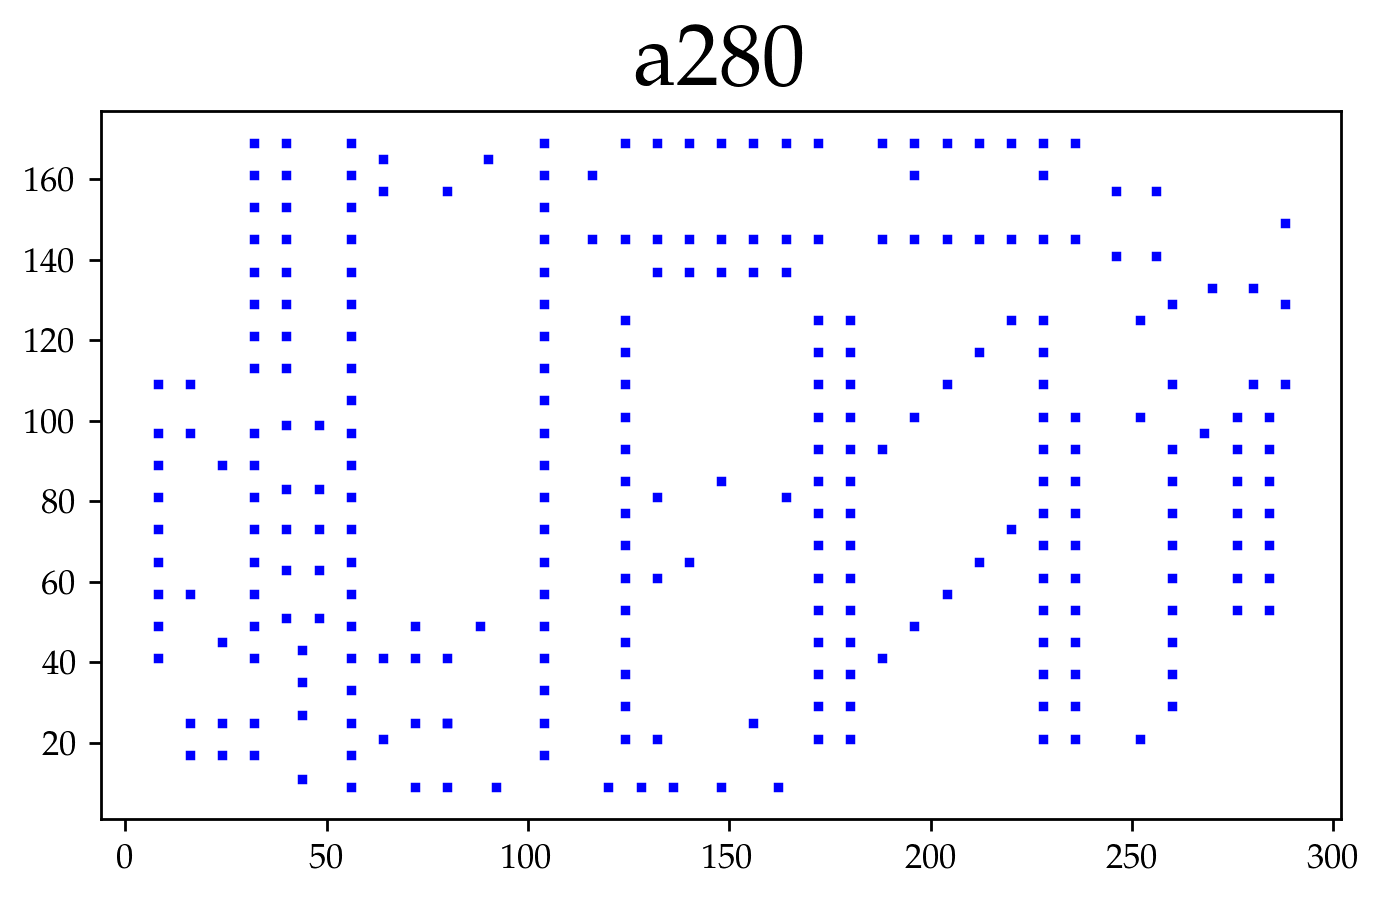
\includegraphics[width=5cm]{../tsplib_euc2d_pictures_of_instances/a280.png}
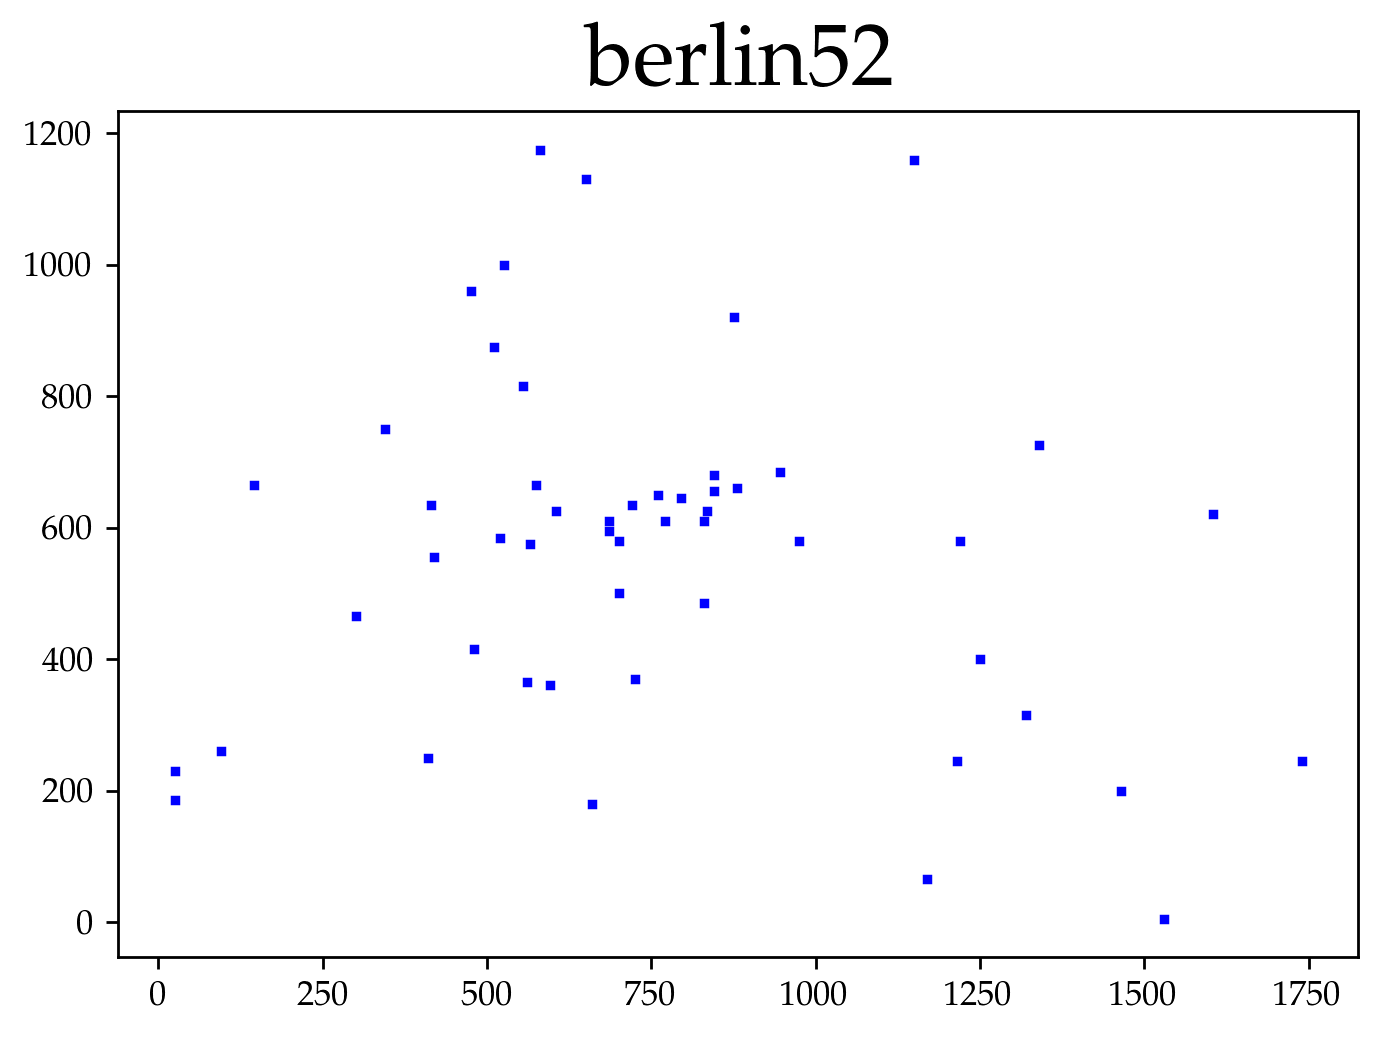
\includegraphics[width=5cm]{../tsplib_euc2d_pictures_of_instances/berlin52.png}
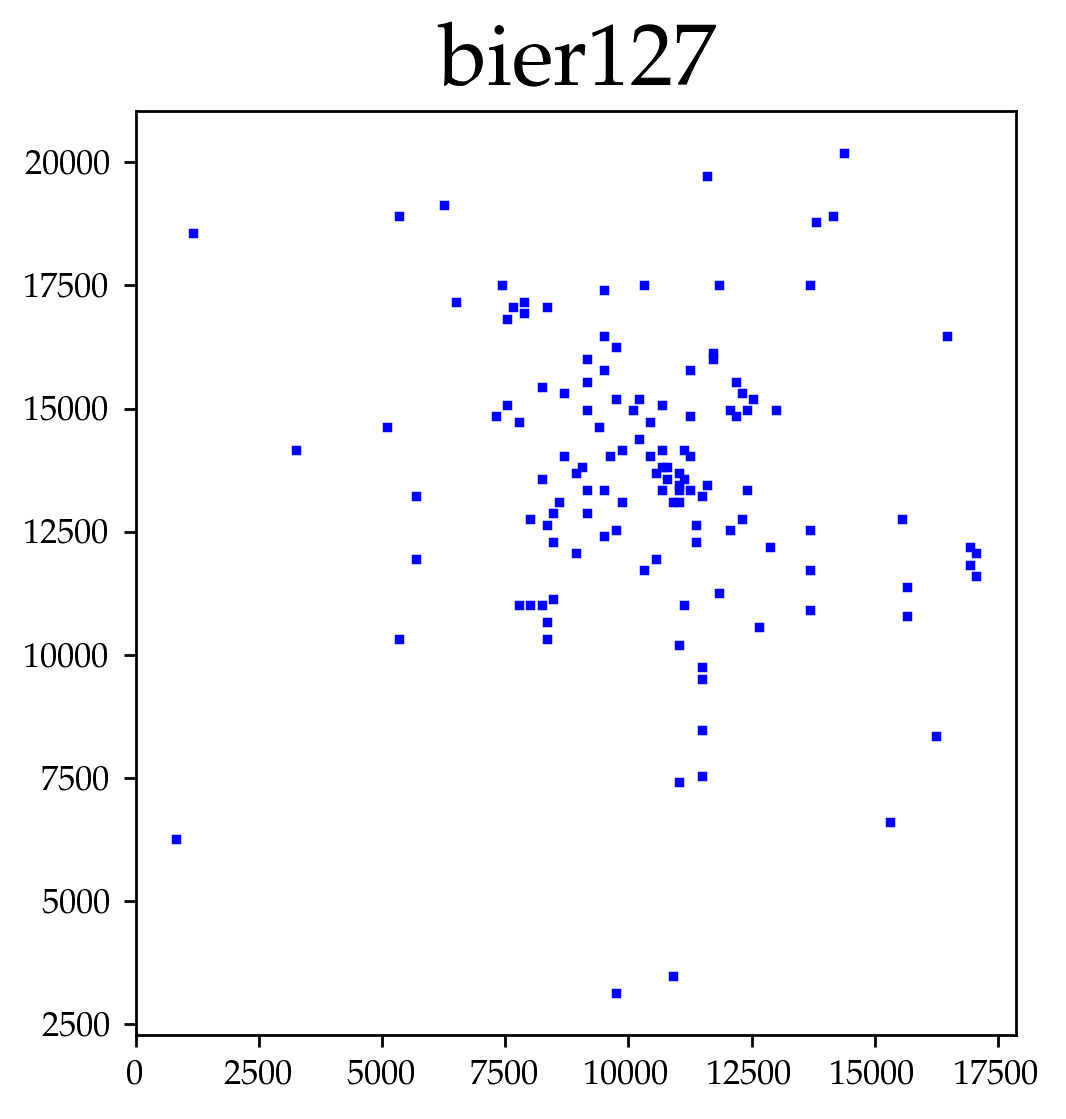
\includegraphics[width=5cm]{../tsplib_euc2d_pictures_of_instances/bier127.png}
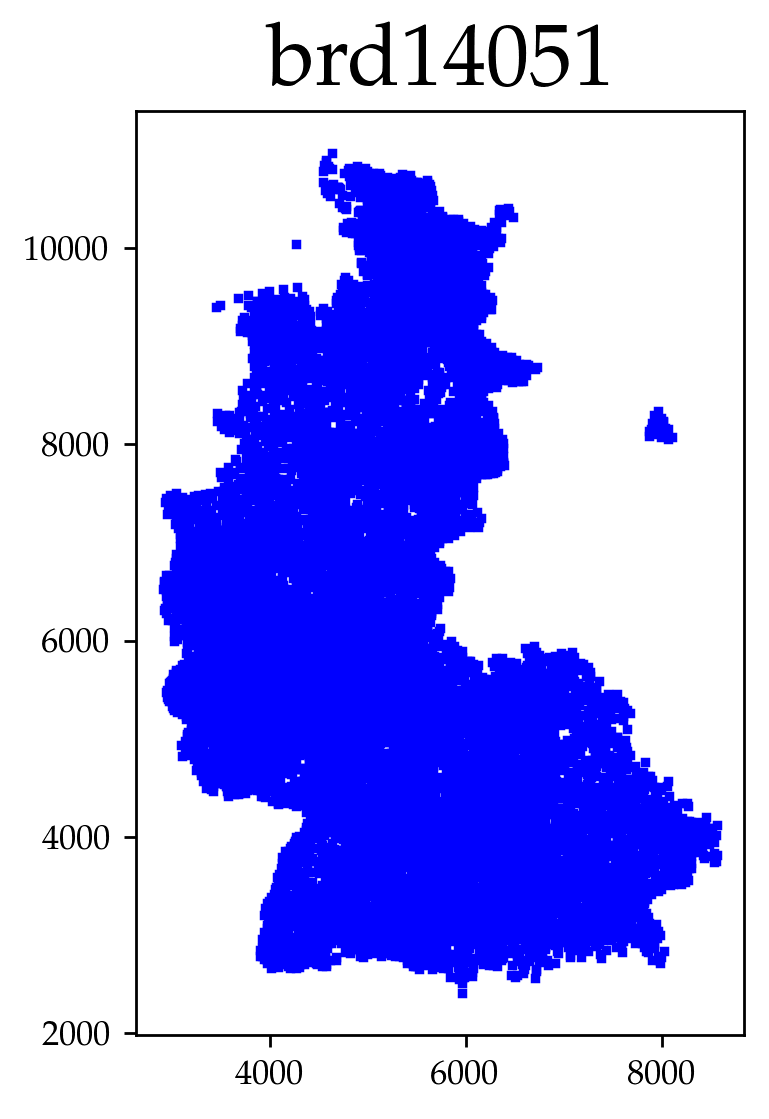
\includegraphics[width=5cm]{../tsplib_euc2d_pictures_of_instances/brd14051.png}
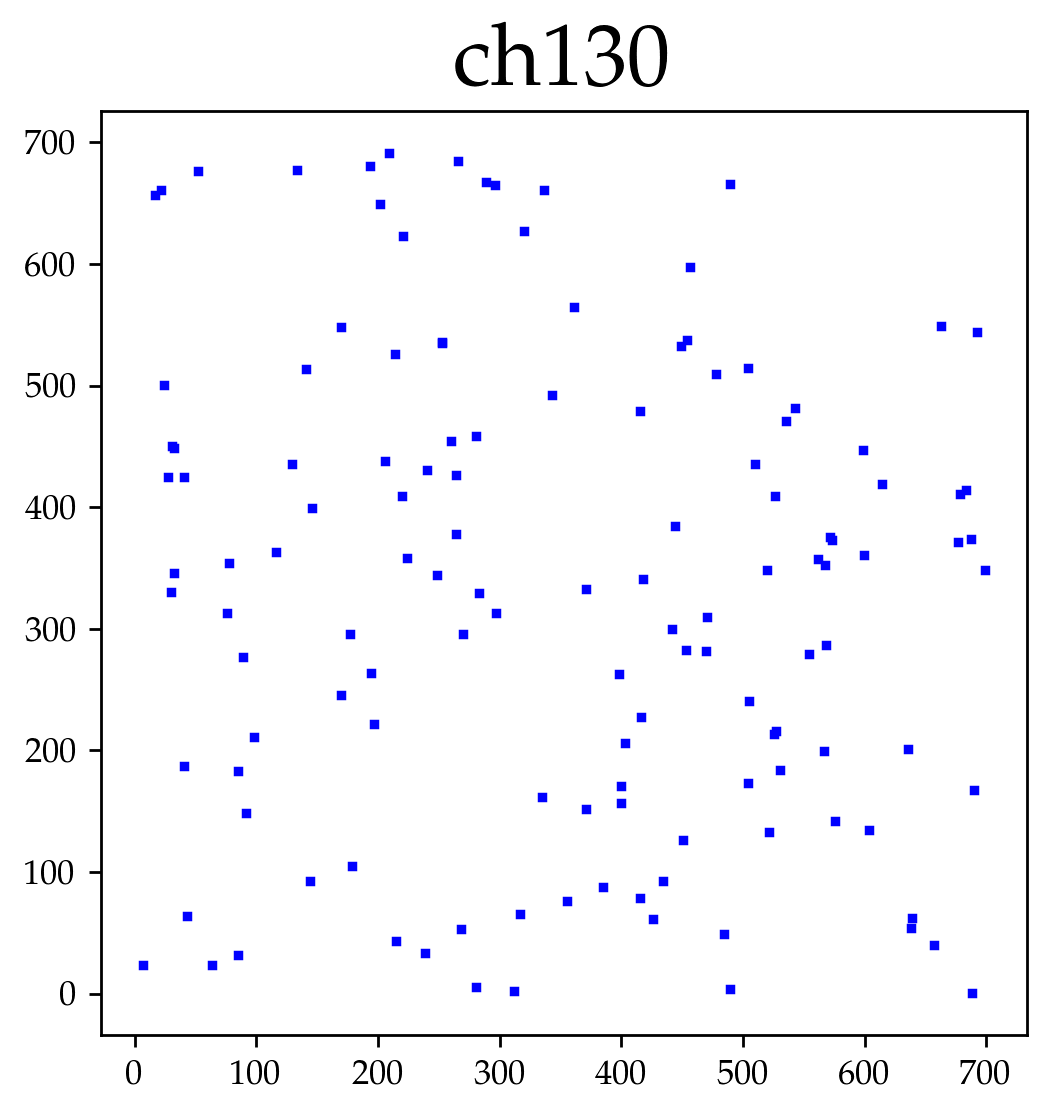
\includegraphics[width=5cm]{../tsplib_euc2d_pictures_of_instances/ch130.png}
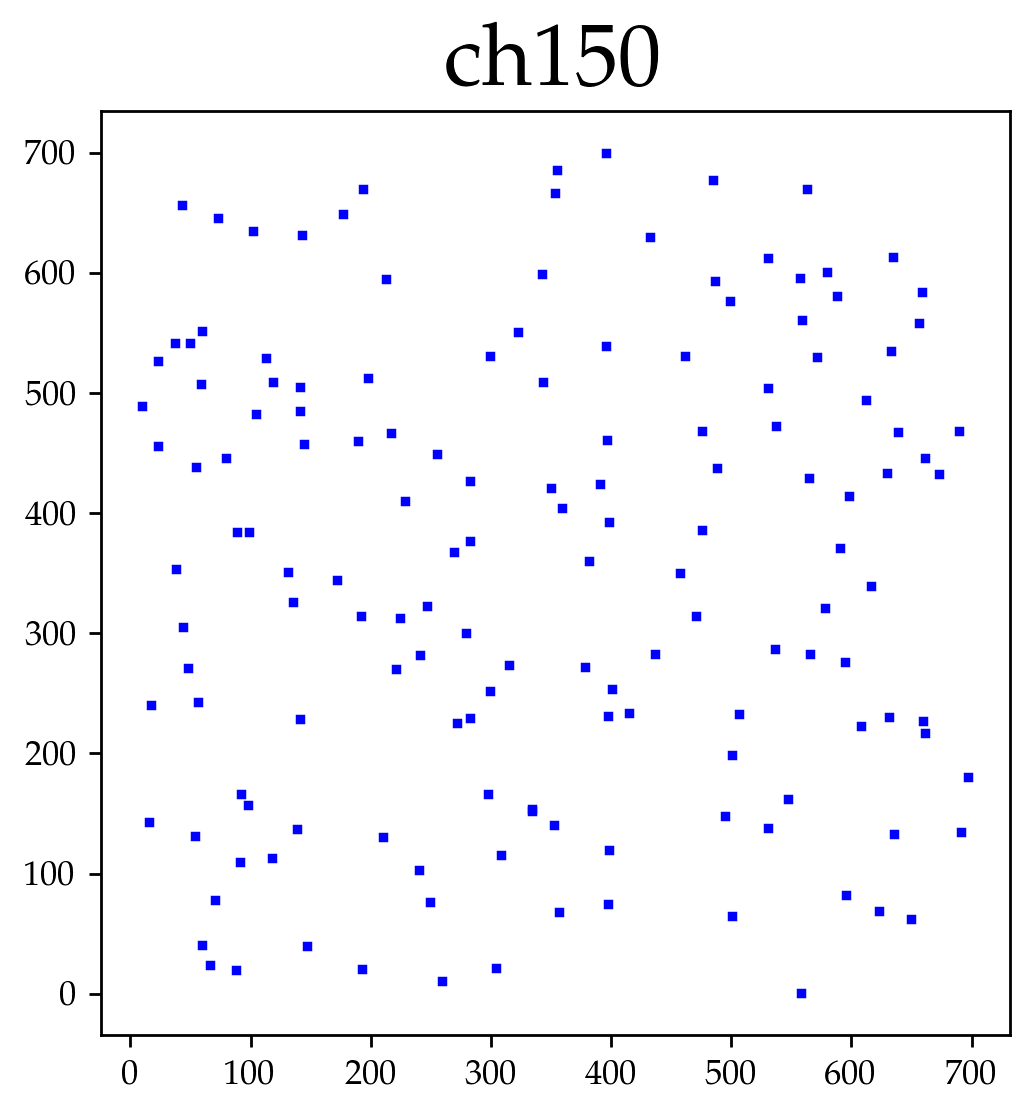
\includegraphics[width=5cm]{../tsplib_euc2d_pictures_of_instances/ch150.png}
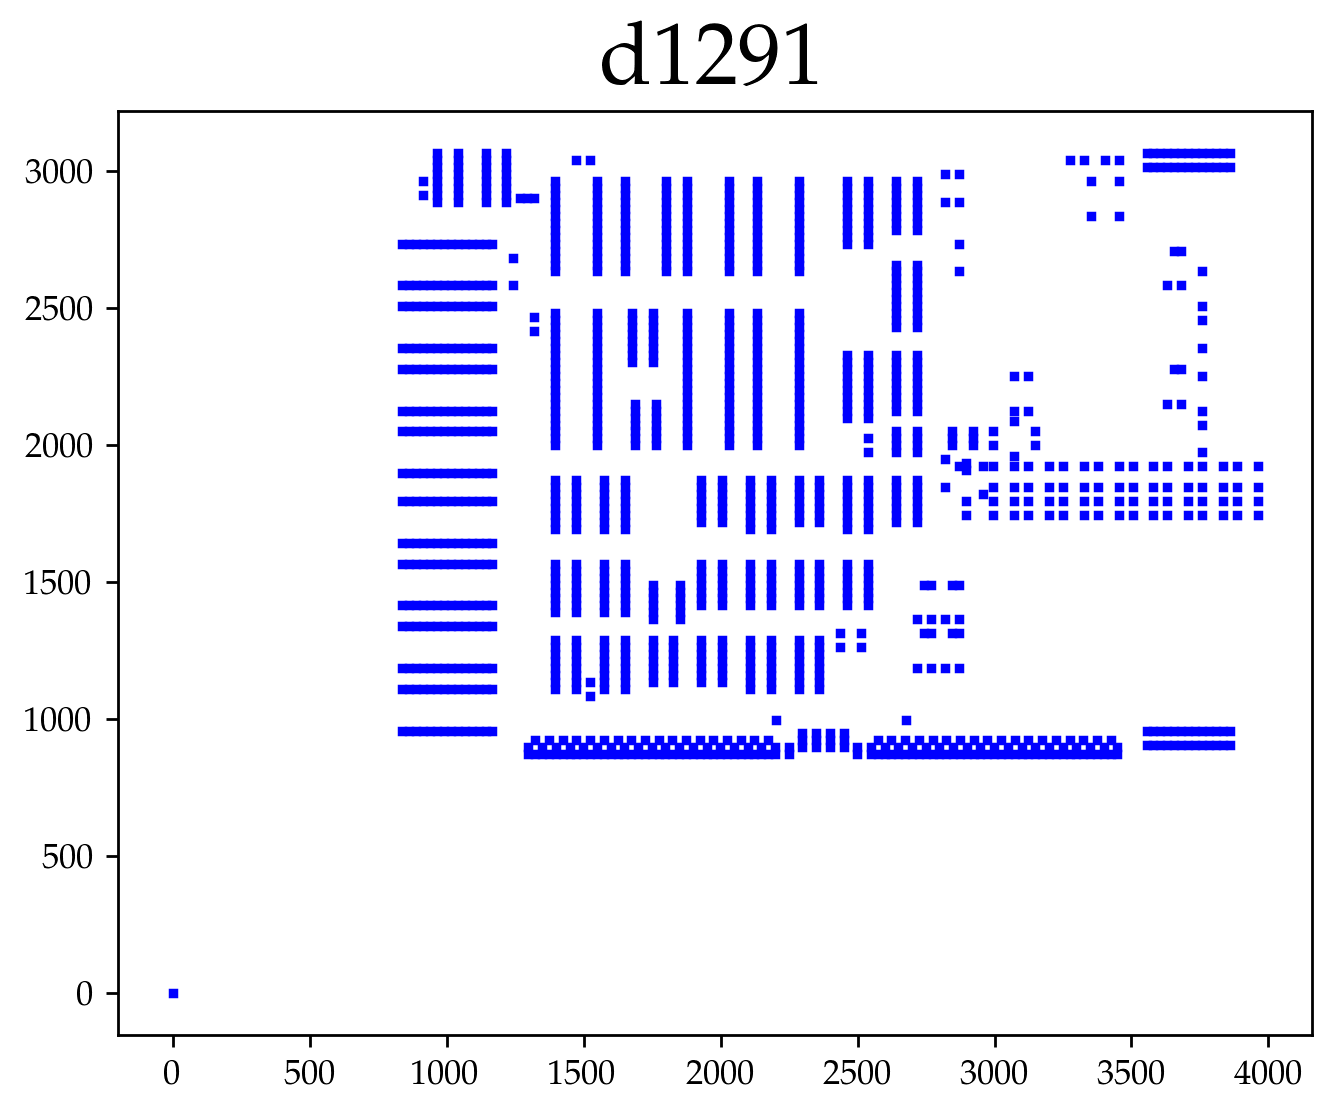
\includegraphics[width=5cm]{../tsplib_euc2d_pictures_of_instances/d1291.png}
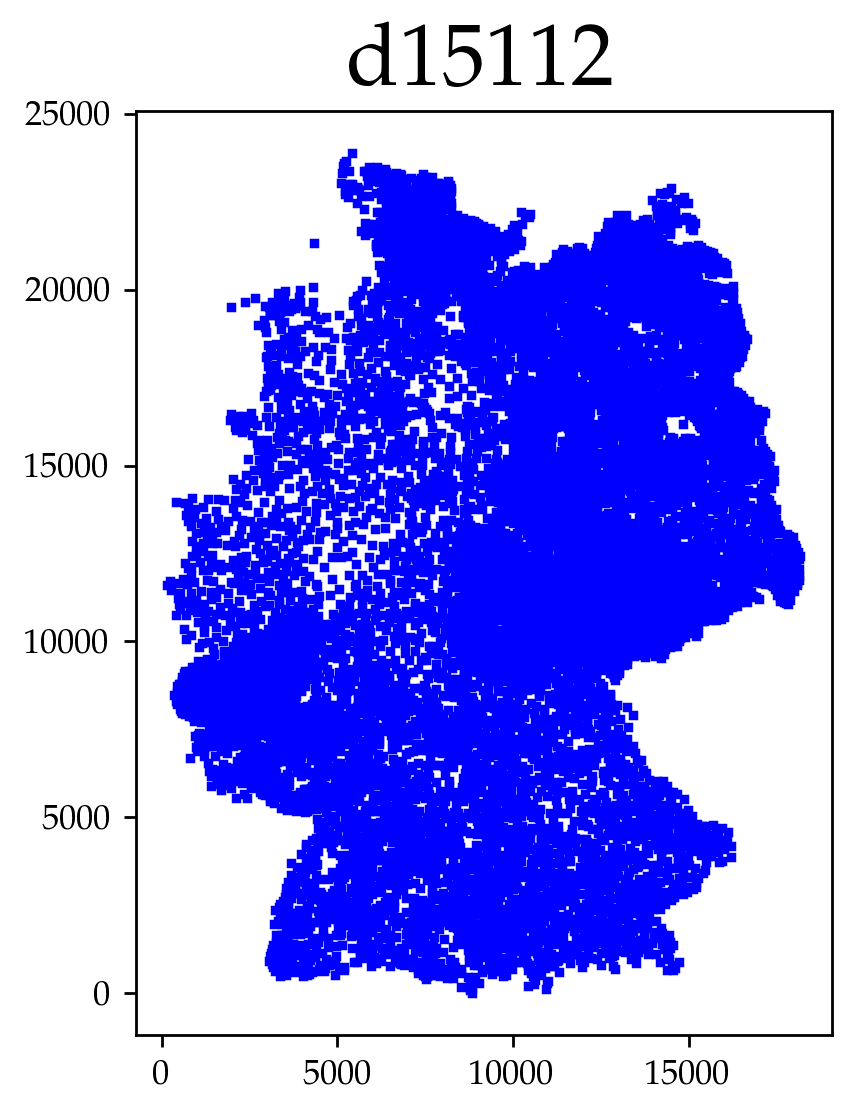
\includegraphics[width=5cm]{../tsplib_euc2d_pictures_of_instances/d15112.png}
\end{figure}

\begin{figure}[H]
\centering

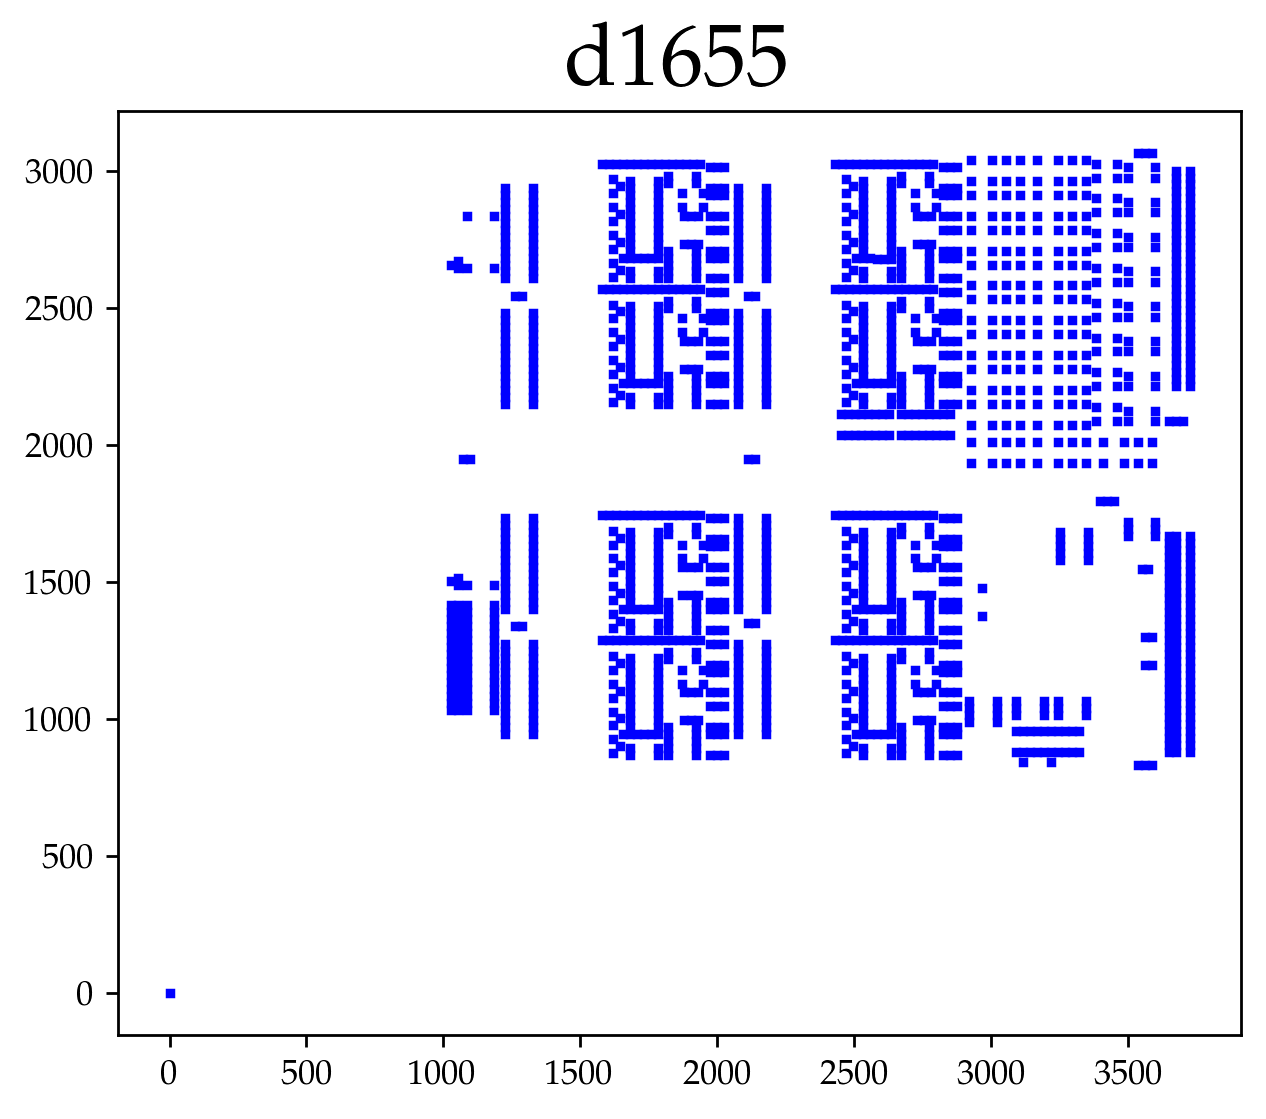
\includegraphics[width=5cm]{../tsplib_euc2d_pictures_of_instances/d1655.png}
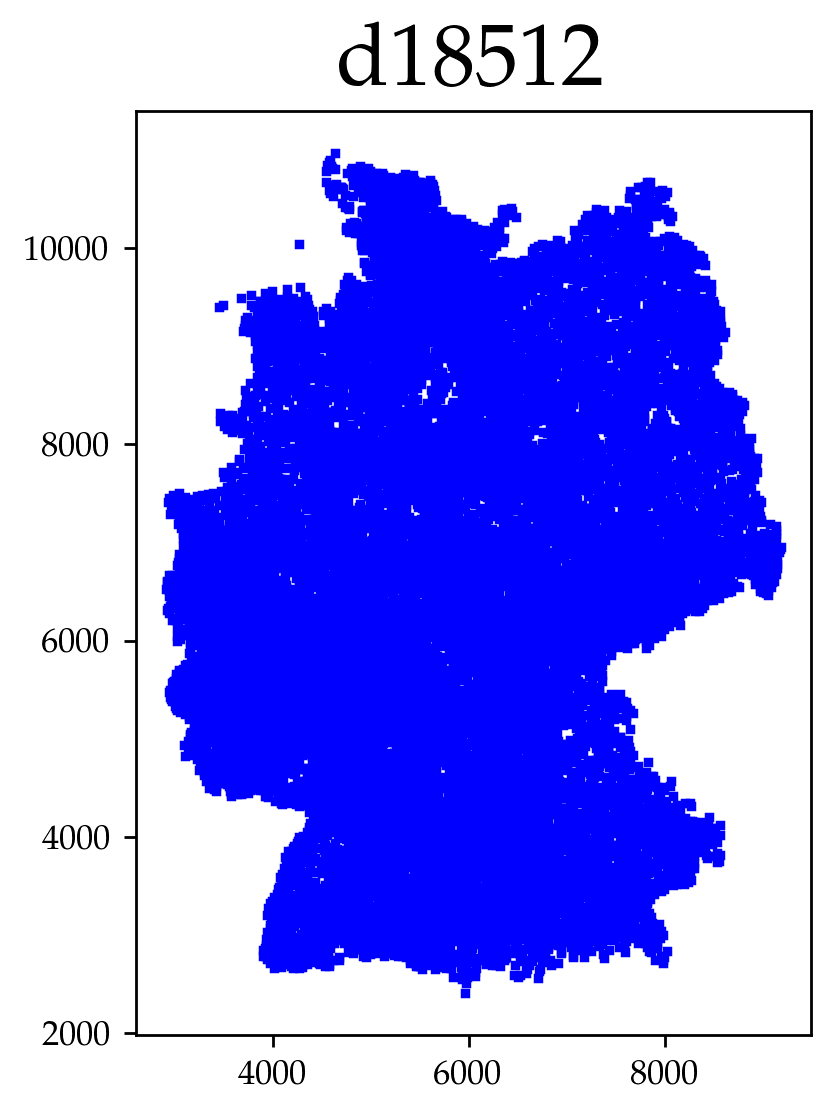
\includegraphics[width=5cm]{../tsplib_euc2d_pictures_of_instances/d18512.png}
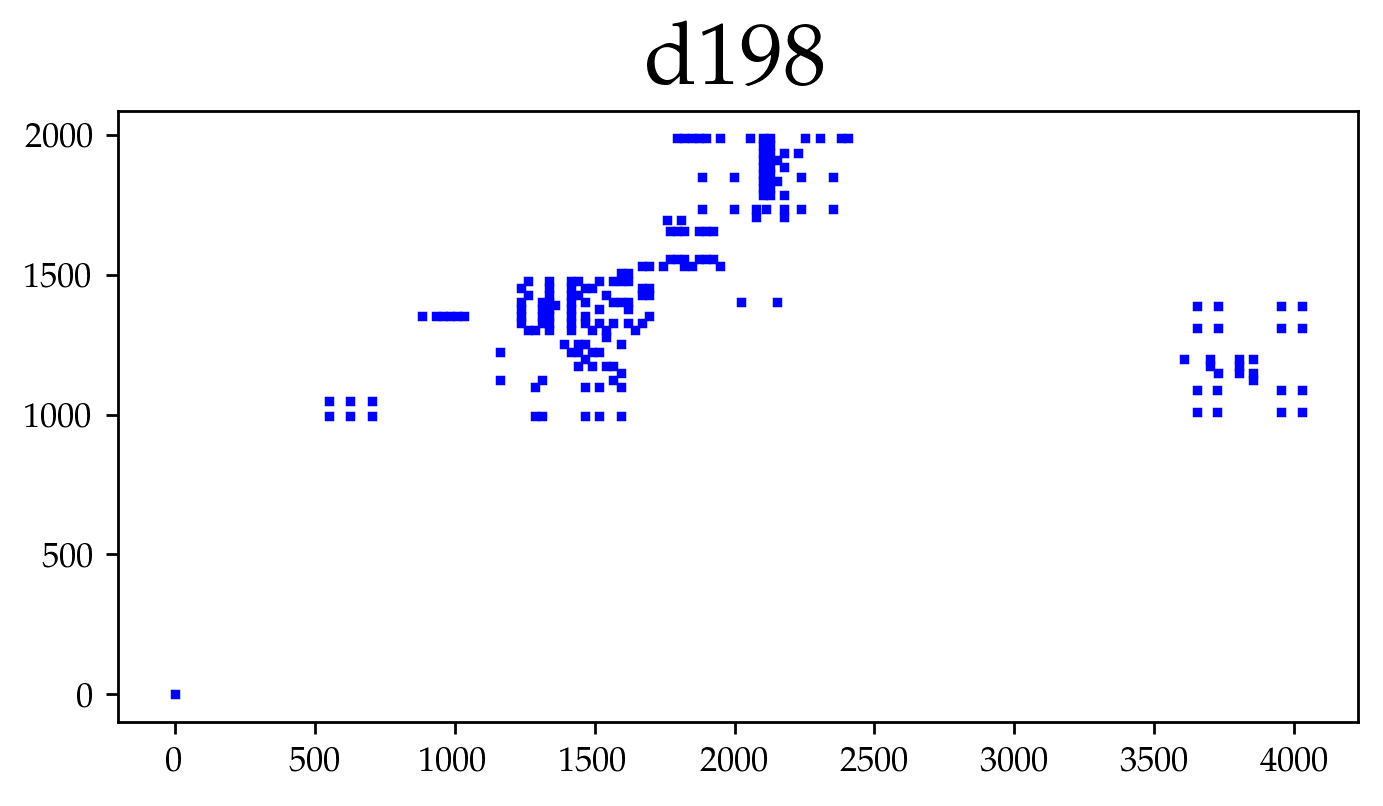
\includegraphics[width=5cm]{../tsplib_euc2d_pictures_of_instances/d198.png}
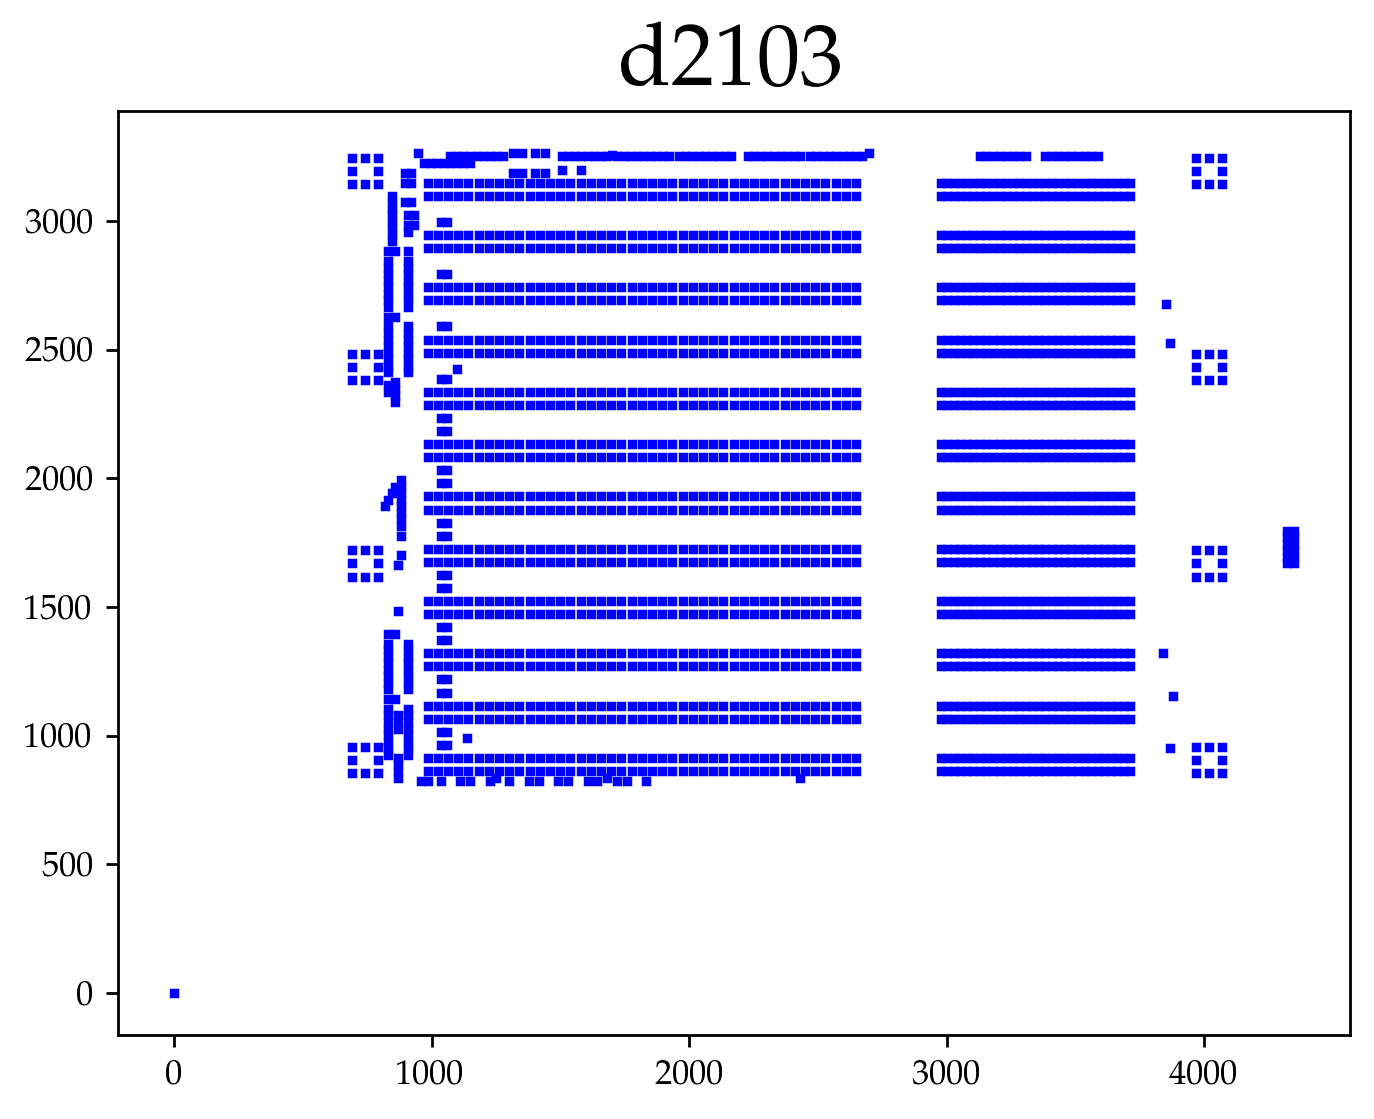
\includegraphics[width=5cm]{../tsplib_euc2d_pictures_of_instances/d2103.png}
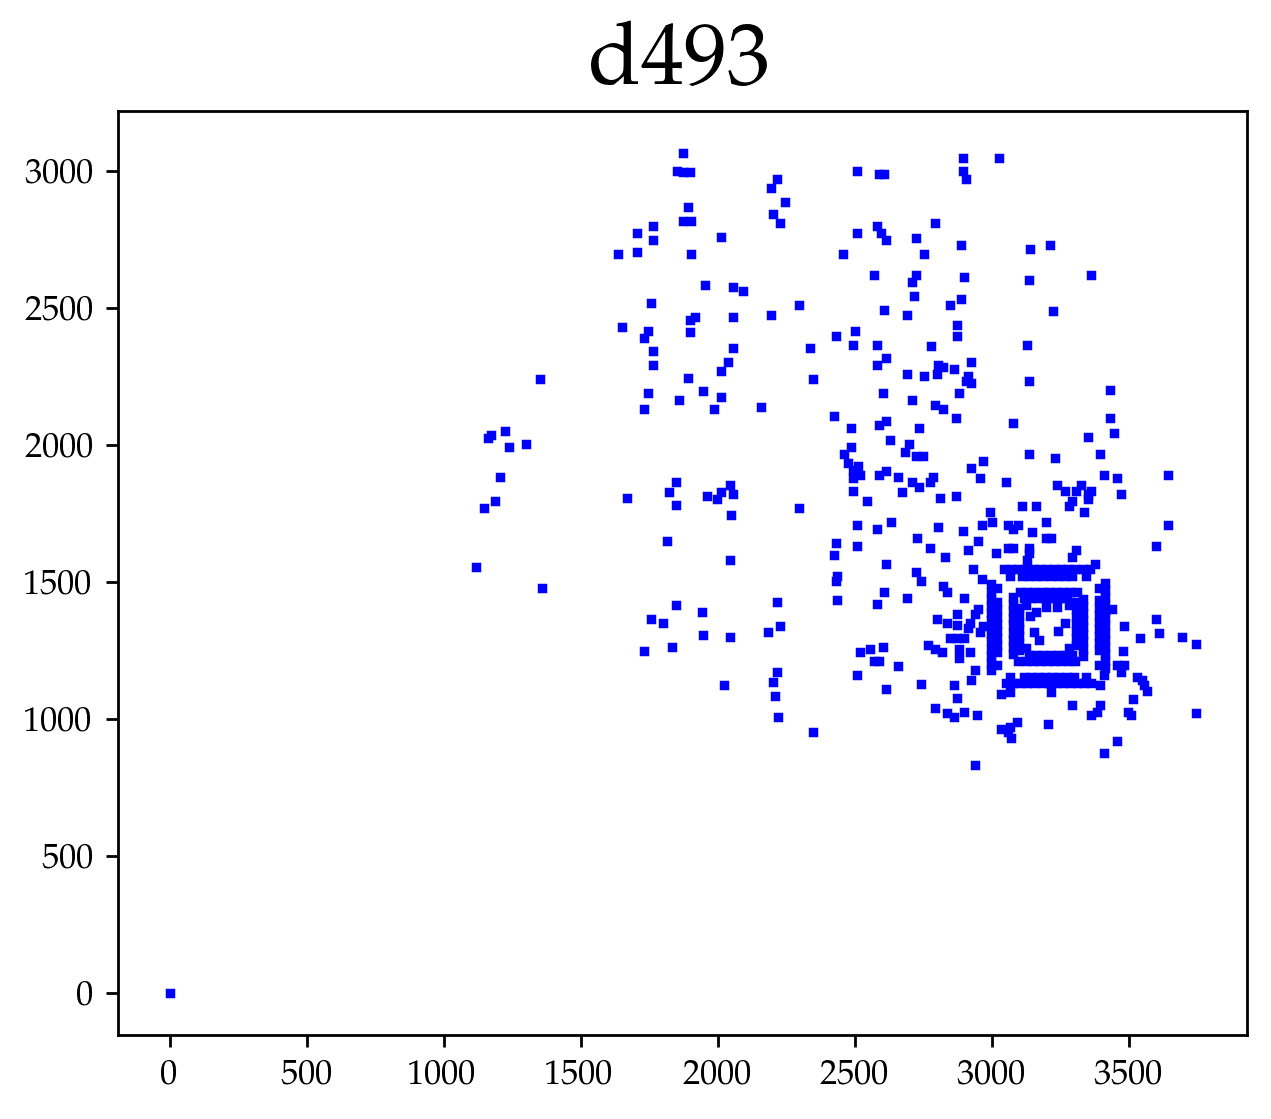
\includegraphics[width=5cm]{../tsplib_euc2d_pictures_of_instances/d493.png}
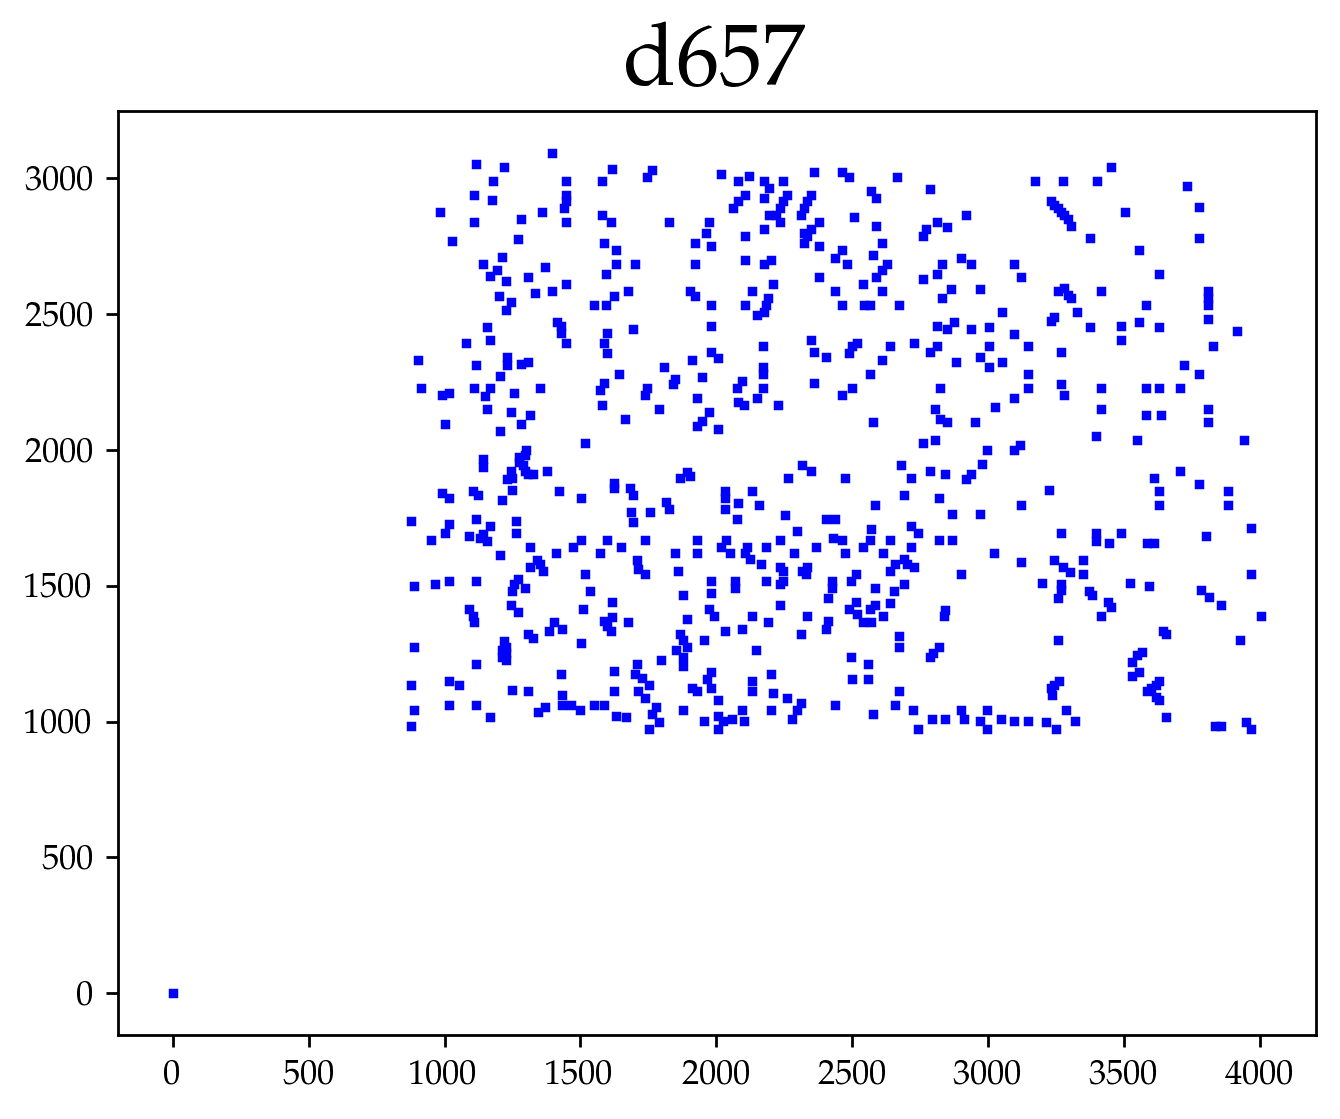
\includegraphics[width=5cm]{../tsplib_euc2d_pictures_of_instances/d657.png}
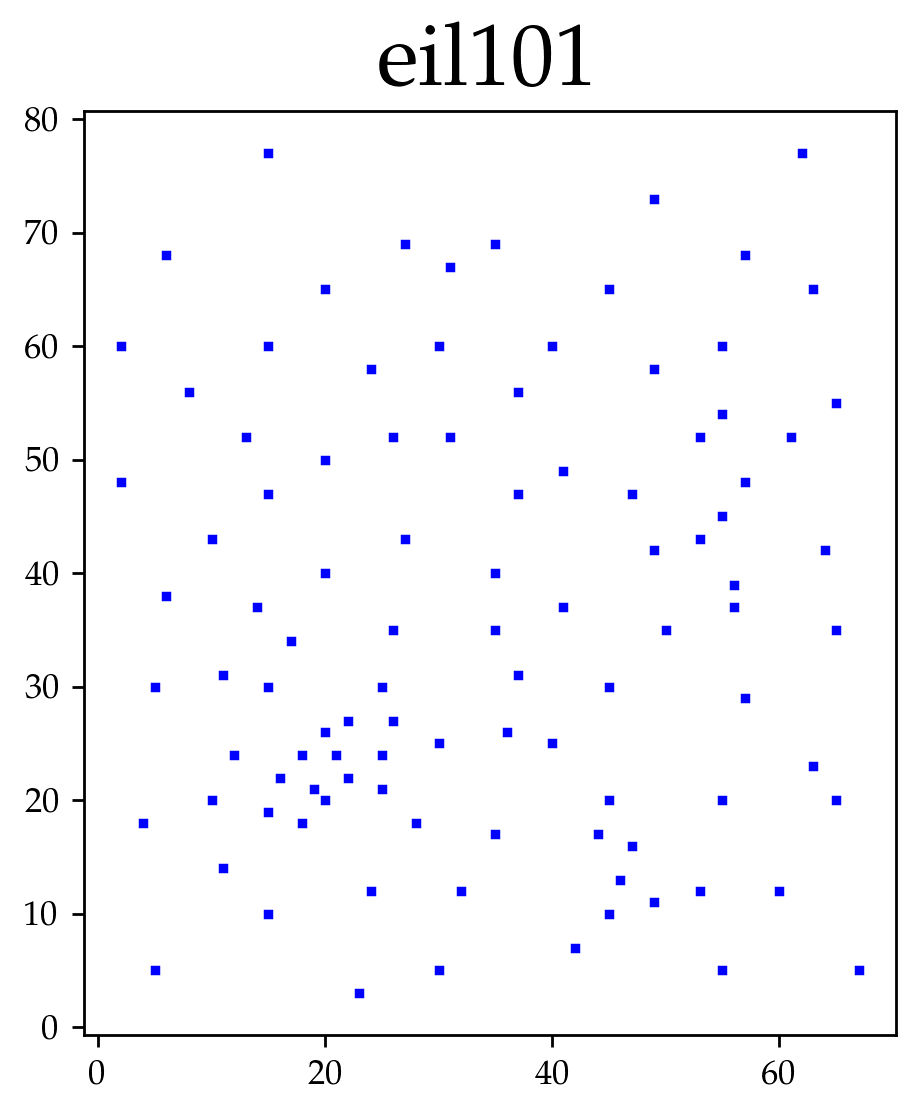
\includegraphics[width=5cm]{../tsplib_euc2d_pictures_of_instances/eil101.png}
\end{figure}

\begin{figure}[H]
\centering
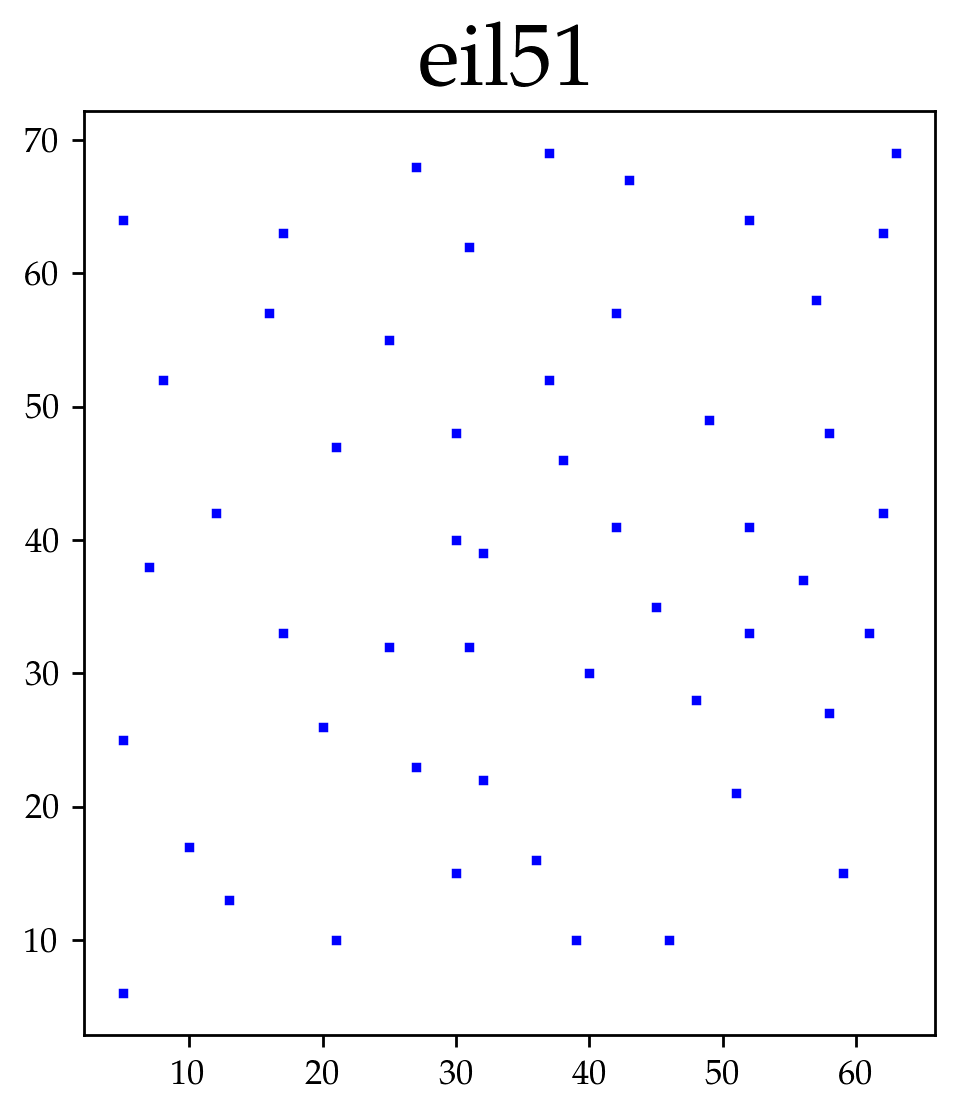
\includegraphics[width=5cm]{../tsplib_euc2d_pictures_of_instances/eil51.png}
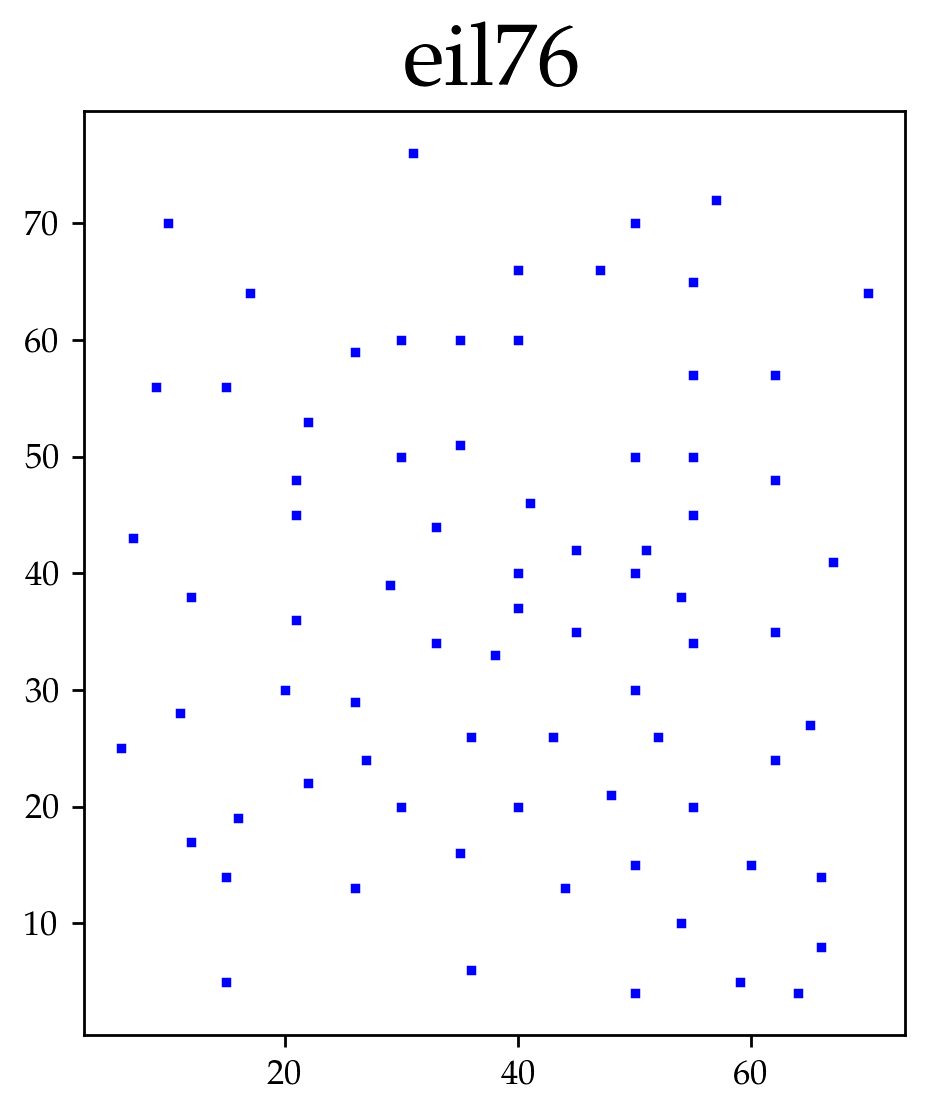
\includegraphics[width=5cm]{../tsplib_euc2d_pictures_of_instances/eil76.png}
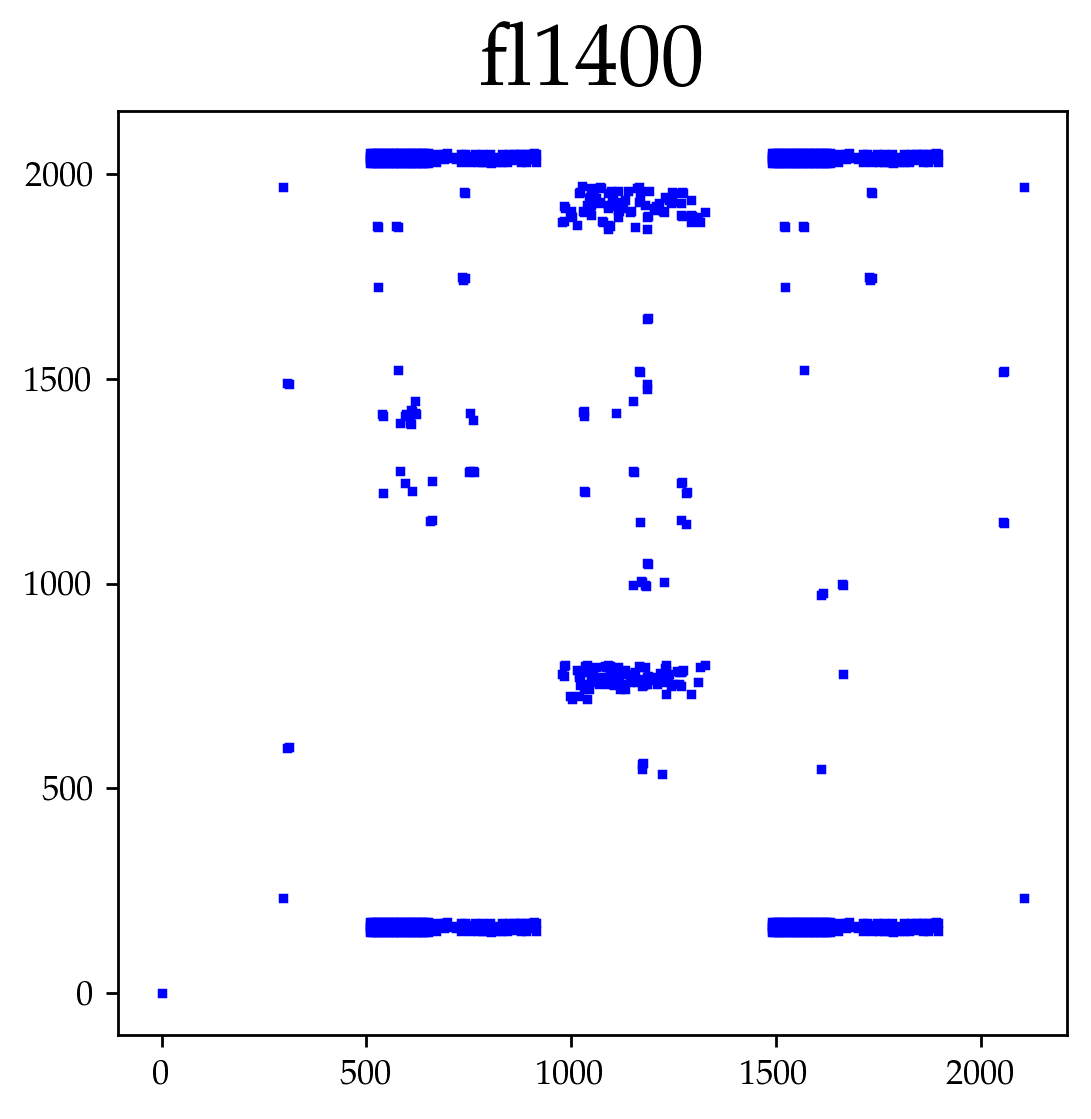
\includegraphics[width=5cm]{../tsplib_euc2d_pictures_of_instances/fl1400.png}
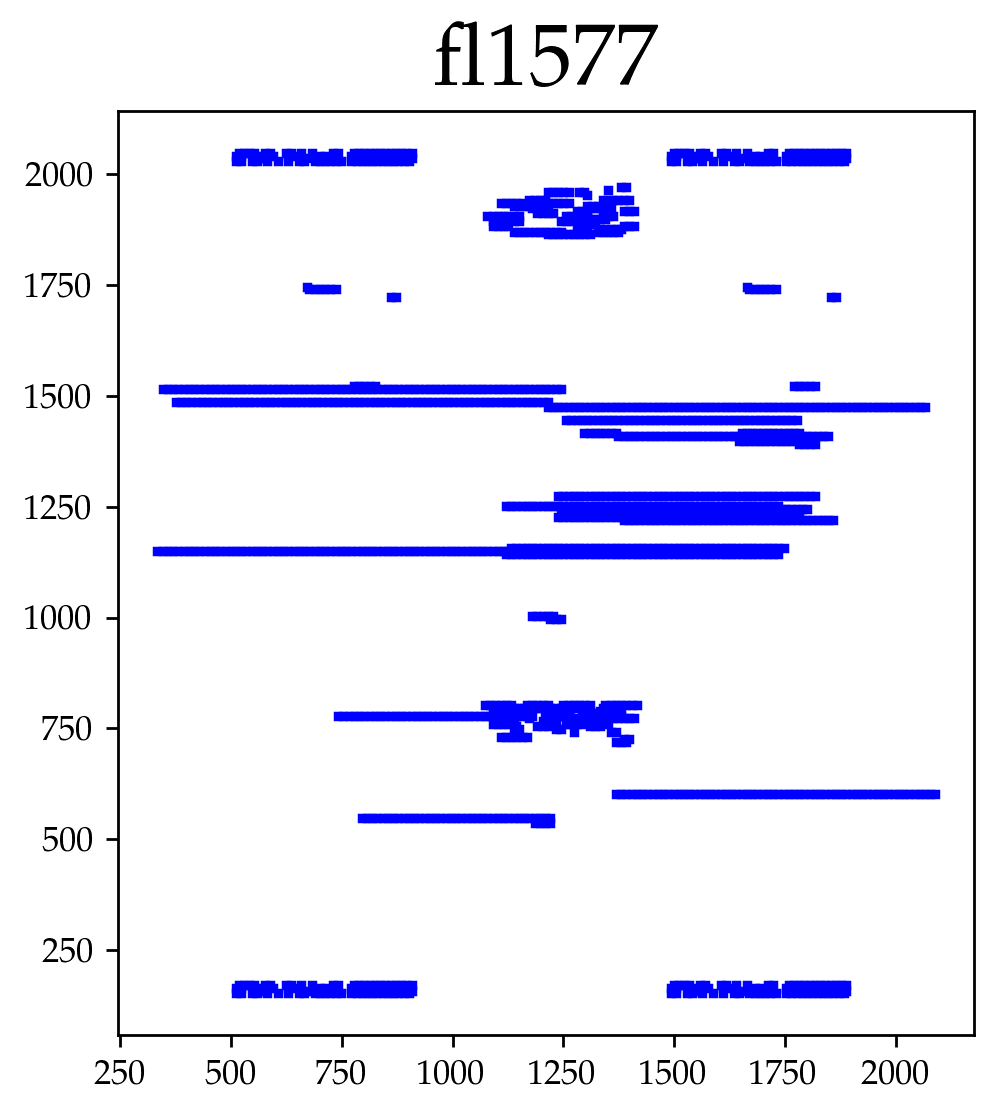
\includegraphics[width=5cm]{../tsplib_euc2d_pictures_of_instances/fl1577.png}
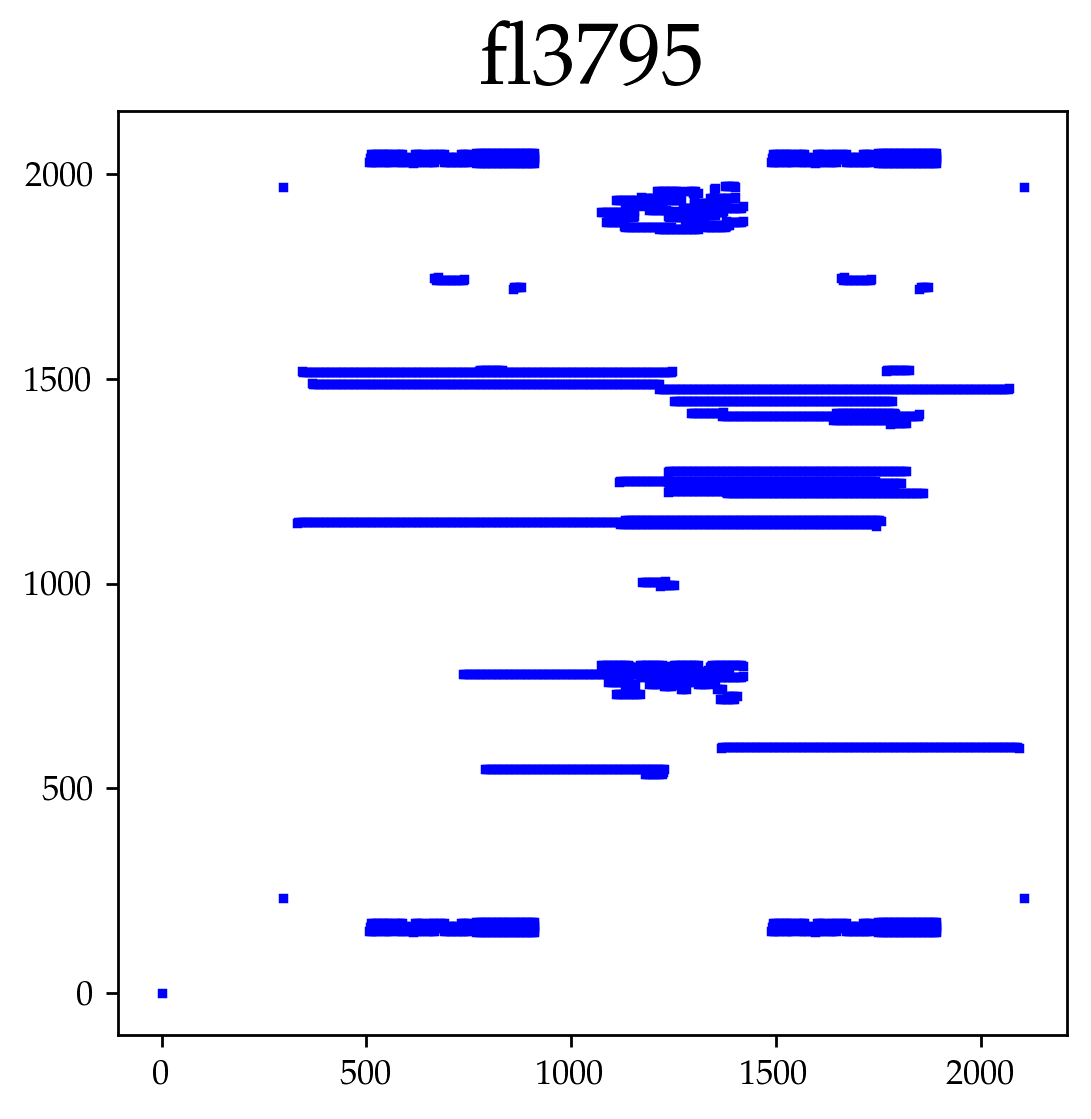
\includegraphics[width=5cm]{../tsplib_euc2d_pictures_of_instances/fl3795.png}
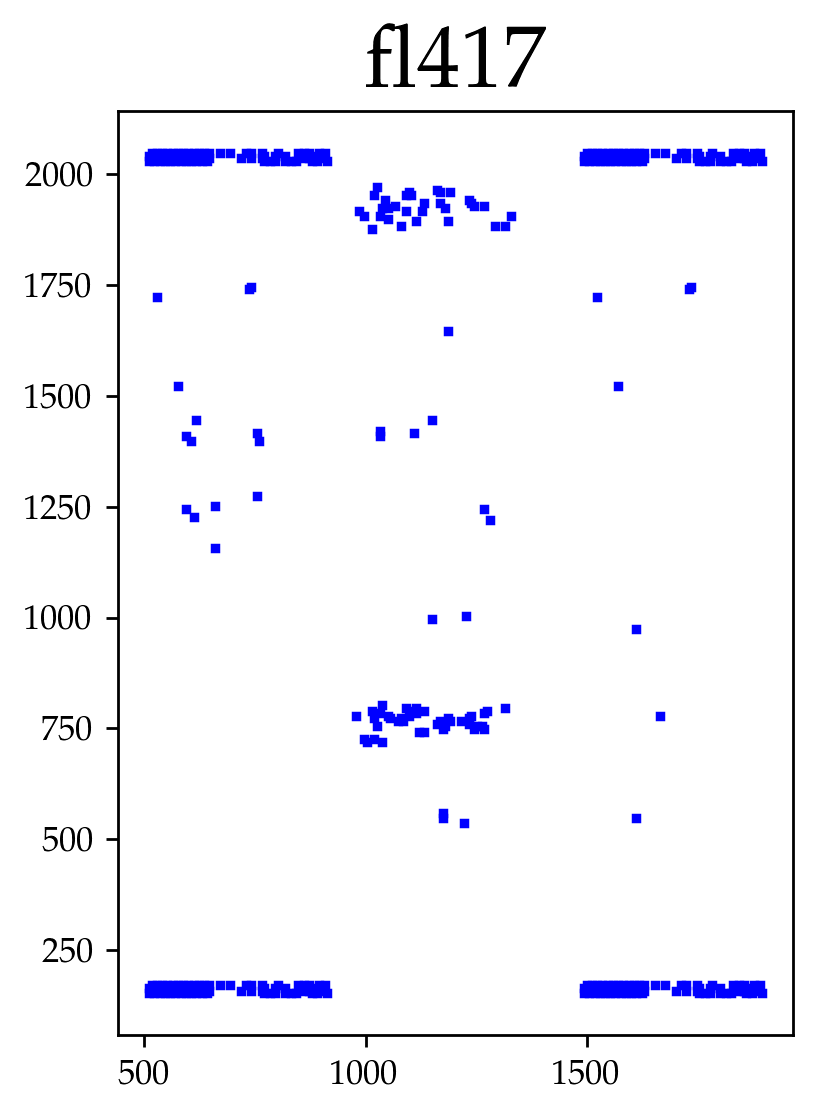
\includegraphics[width=5cm]{../tsplib_euc2d_pictures_of_instances/fl417.png}
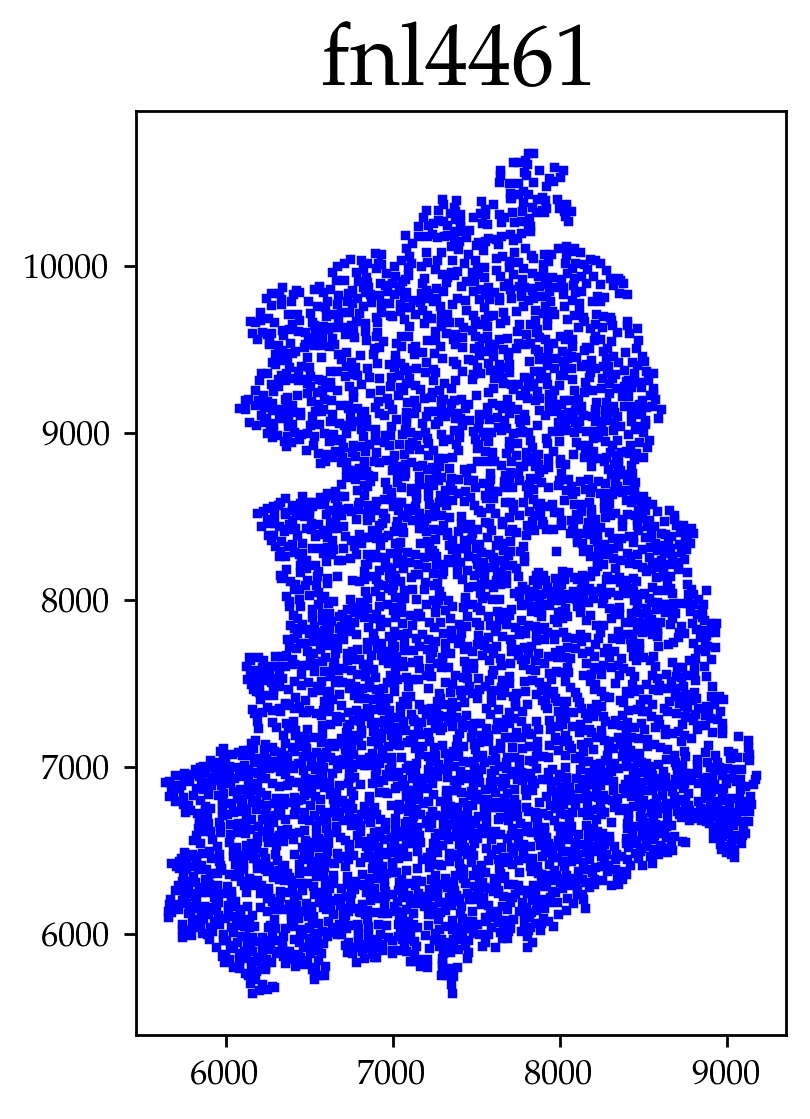
\includegraphics[width=5cm]{../tsplib_euc2d_pictures_of_instances/fnl4461.png}

\end{figure}

\begin{figure}[H]
\centering
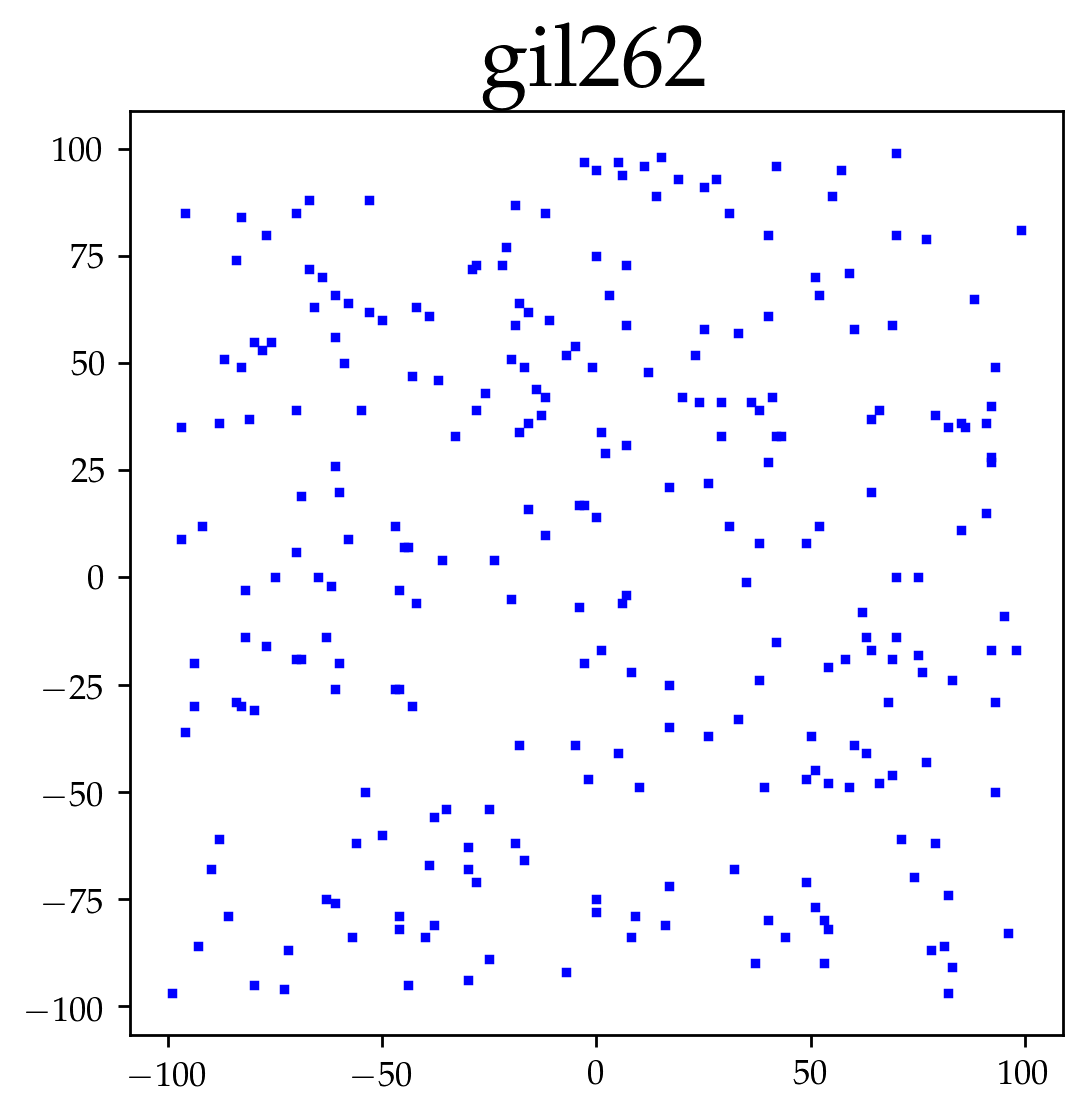
\includegraphics[width=5cm]{../tsplib_euc2d_pictures_of_instances/gil262.png}
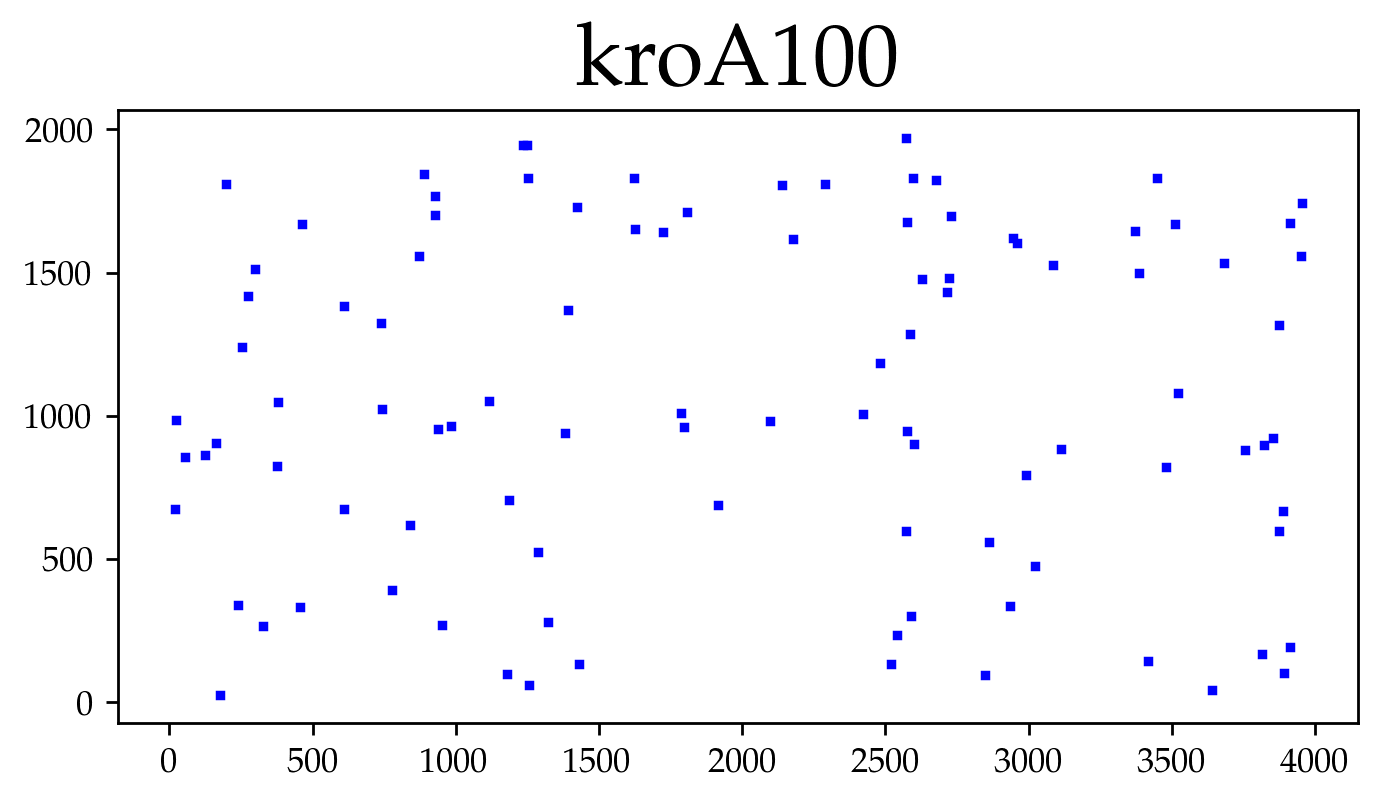
\includegraphics[width=5cm]{../tsplib_euc2d_pictures_of_instances/kroA100.png}
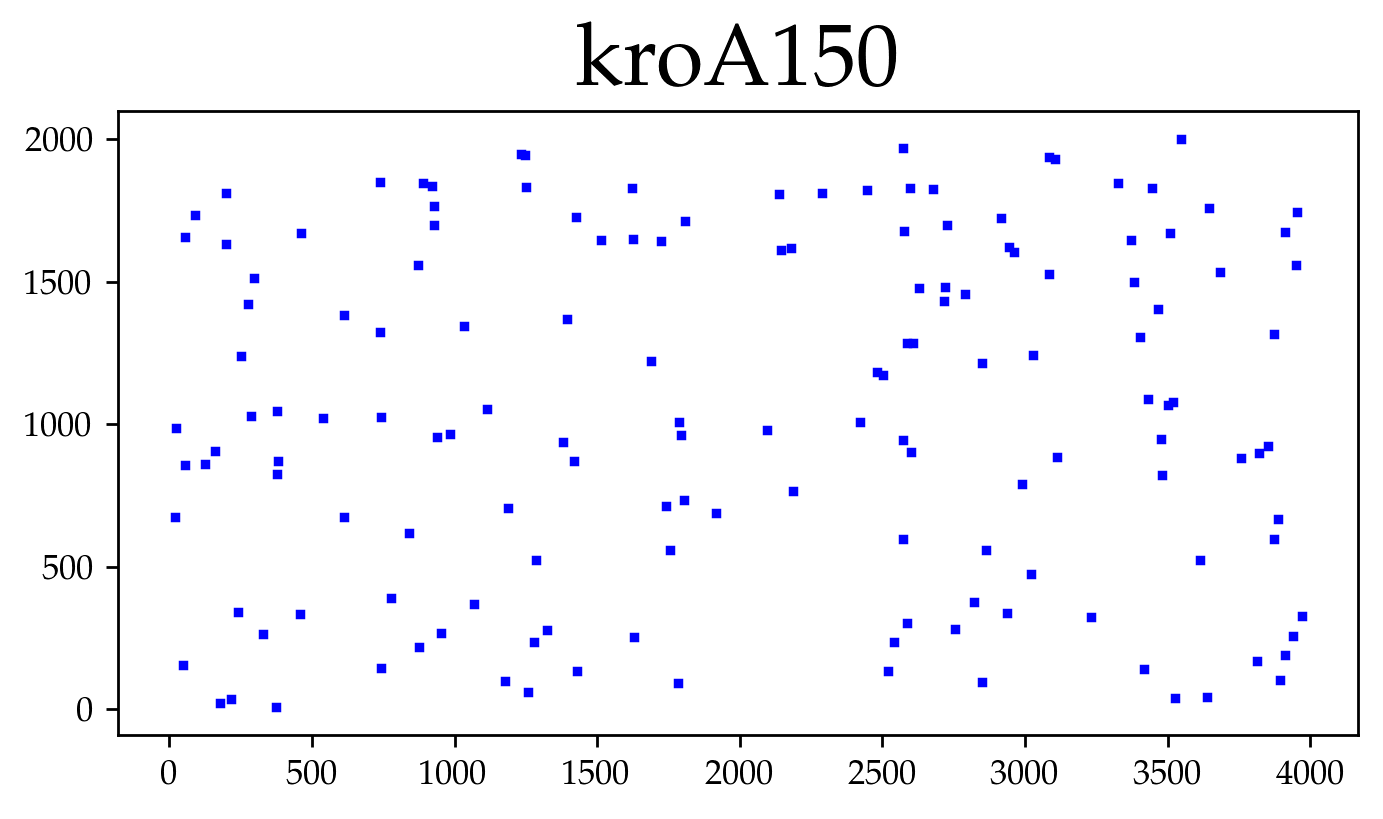
\includegraphics[width=5cm]{../tsplib_euc2d_pictures_of_instances/kroA150.png}
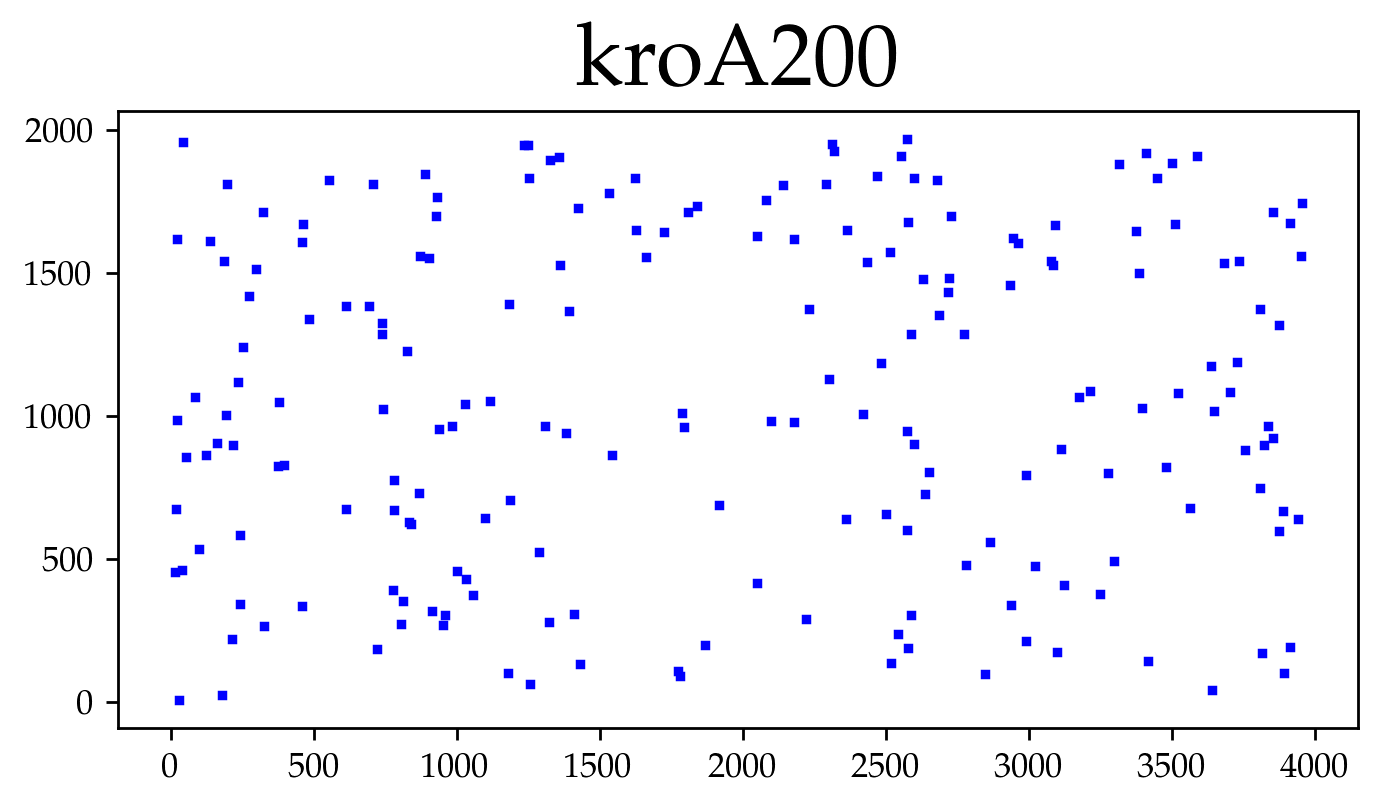
\includegraphics[width=5cm]{../tsplib_euc2d_pictures_of_instances/kroA200.png}
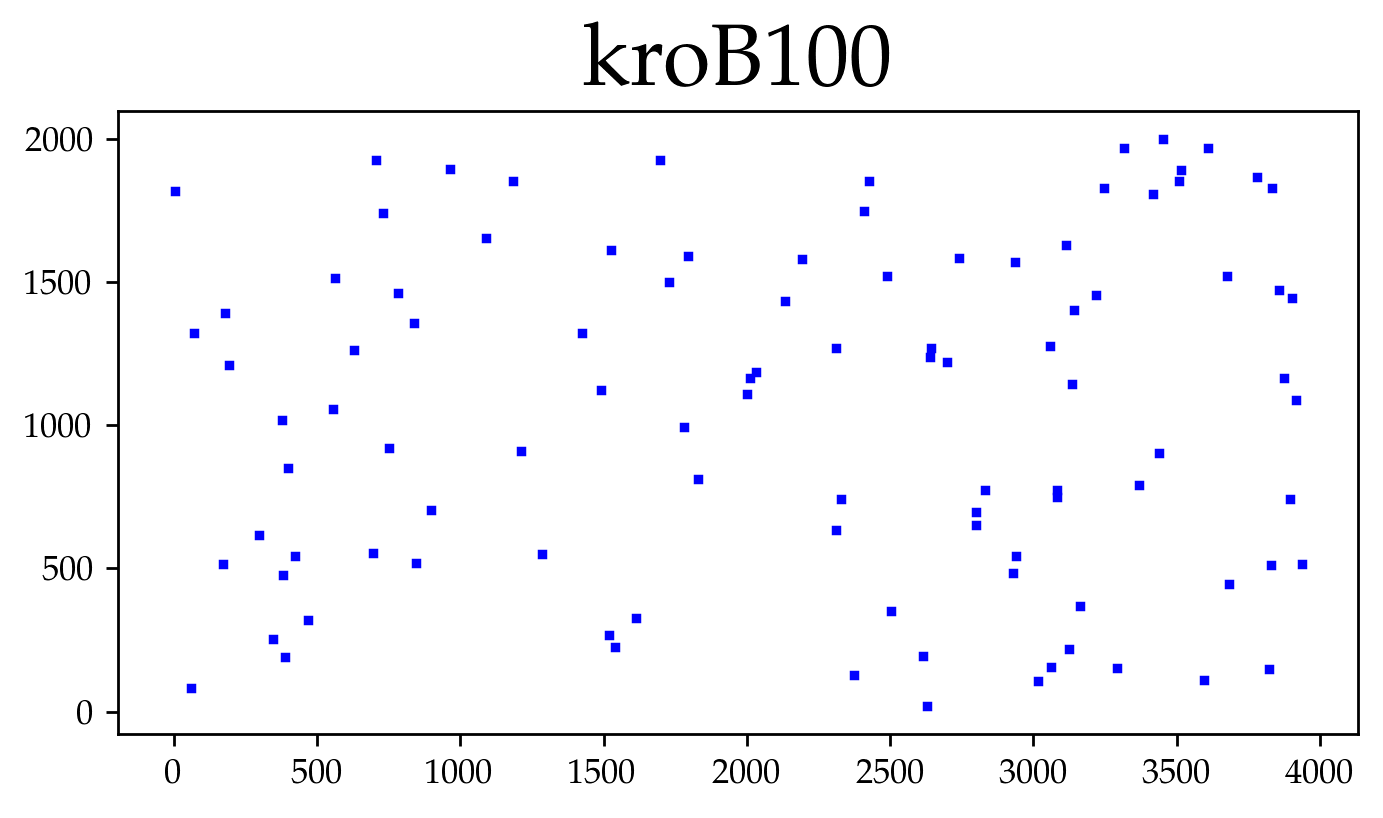
\includegraphics[width=5cm]{../tsplib_euc2d_pictures_of_instances/kroB100.png}
\end{figure}

\begin{figure}[H]
\centering

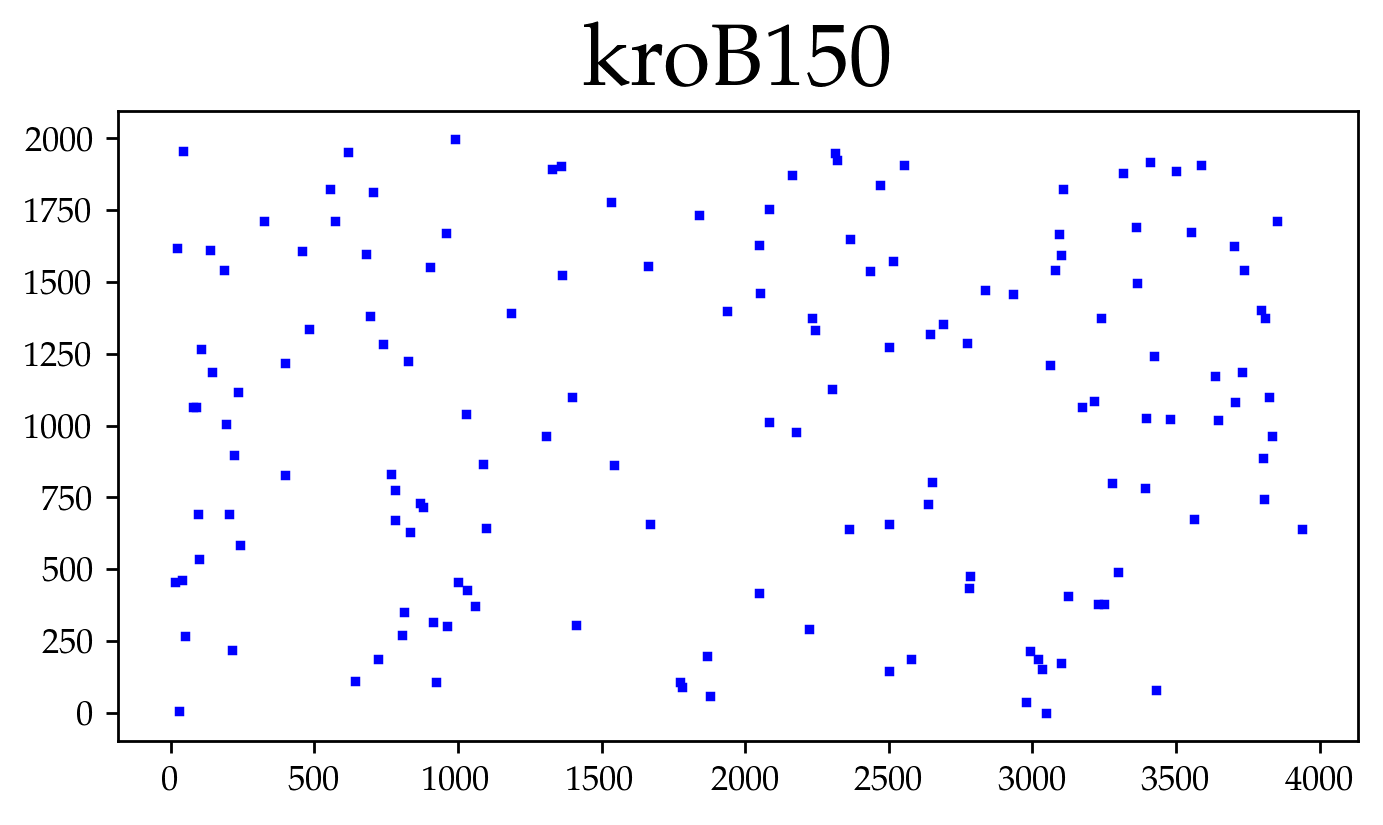
\includegraphics[width=5cm]{../tsplib_euc2d_pictures_of_instances/kroB150.png}
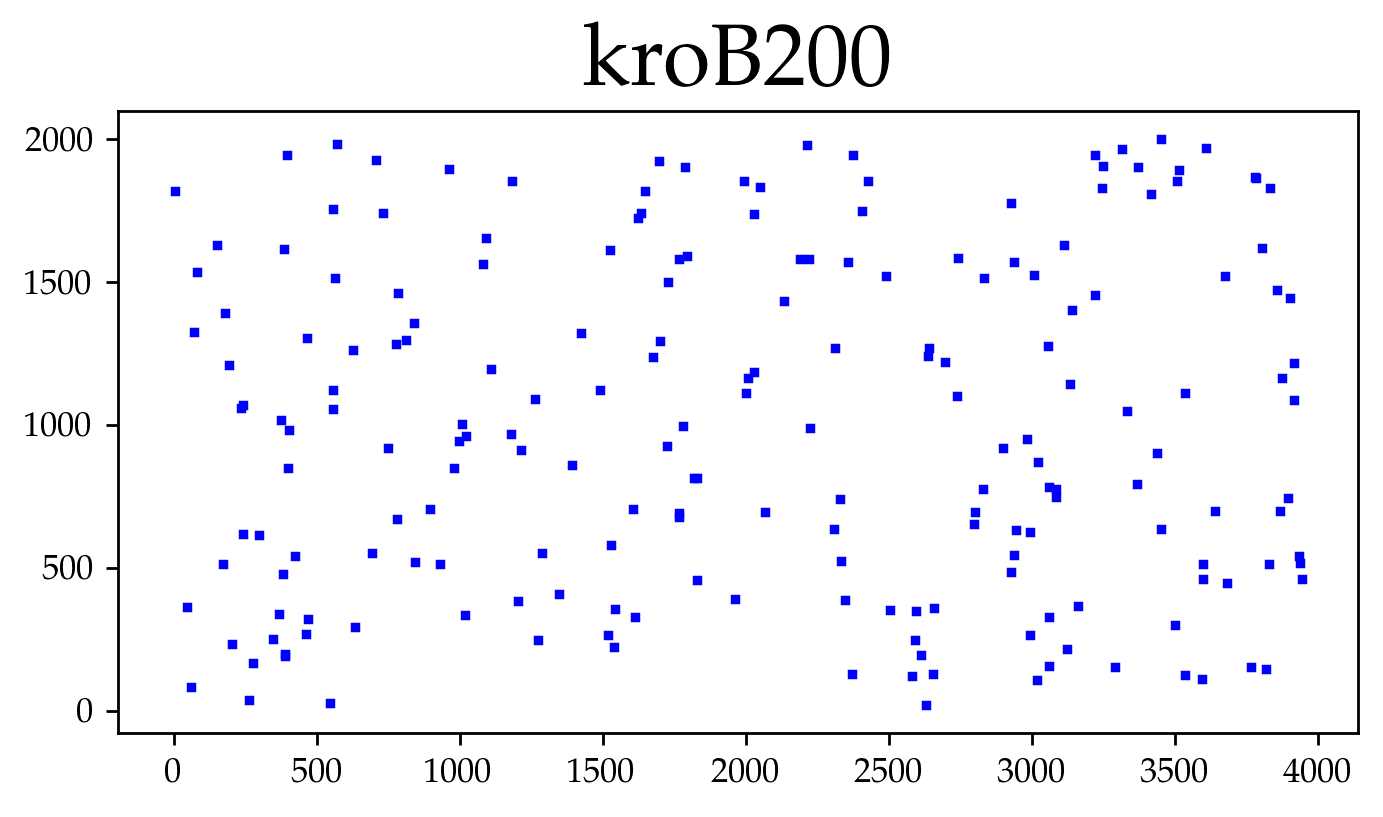
\includegraphics[width=5cm]{../tsplib_euc2d_pictures_of_instances/kroB200.png}
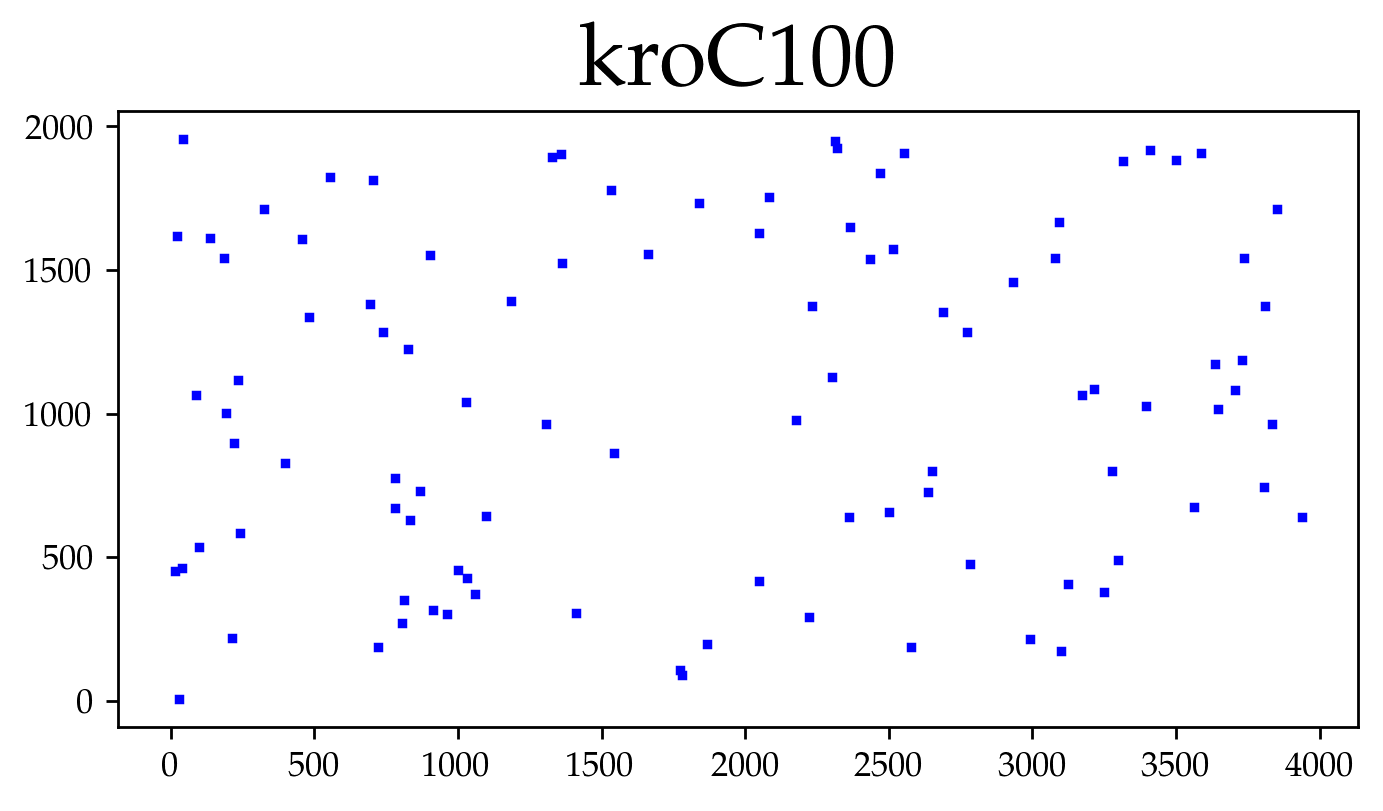
\includegraphics[width=5cm]{../tsplib_euc2d_pictures_of_instances/kroC100.png}
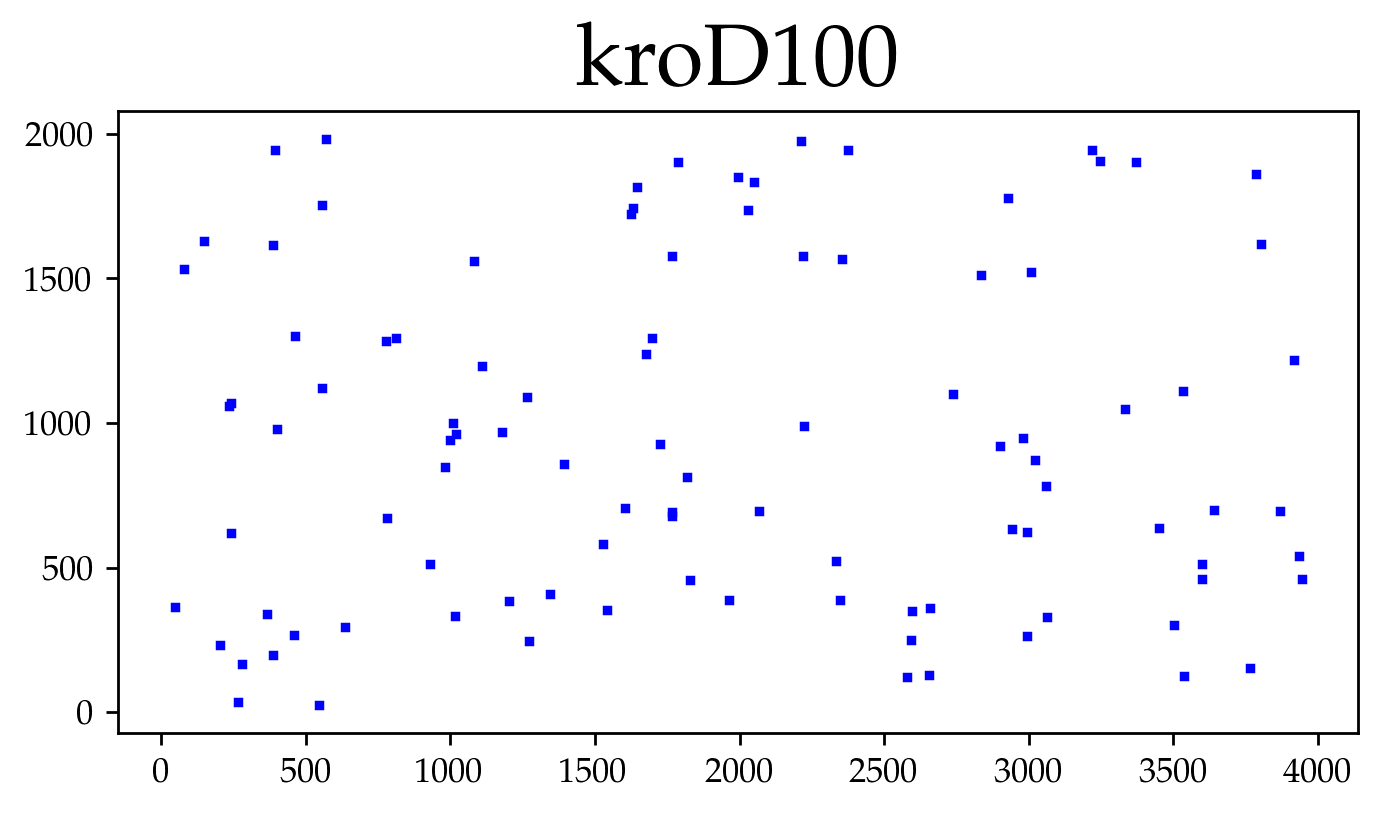
\includegraphics[width=5cm]{../tsplib_euc2d_pictures_of_instances/kroD100.png}
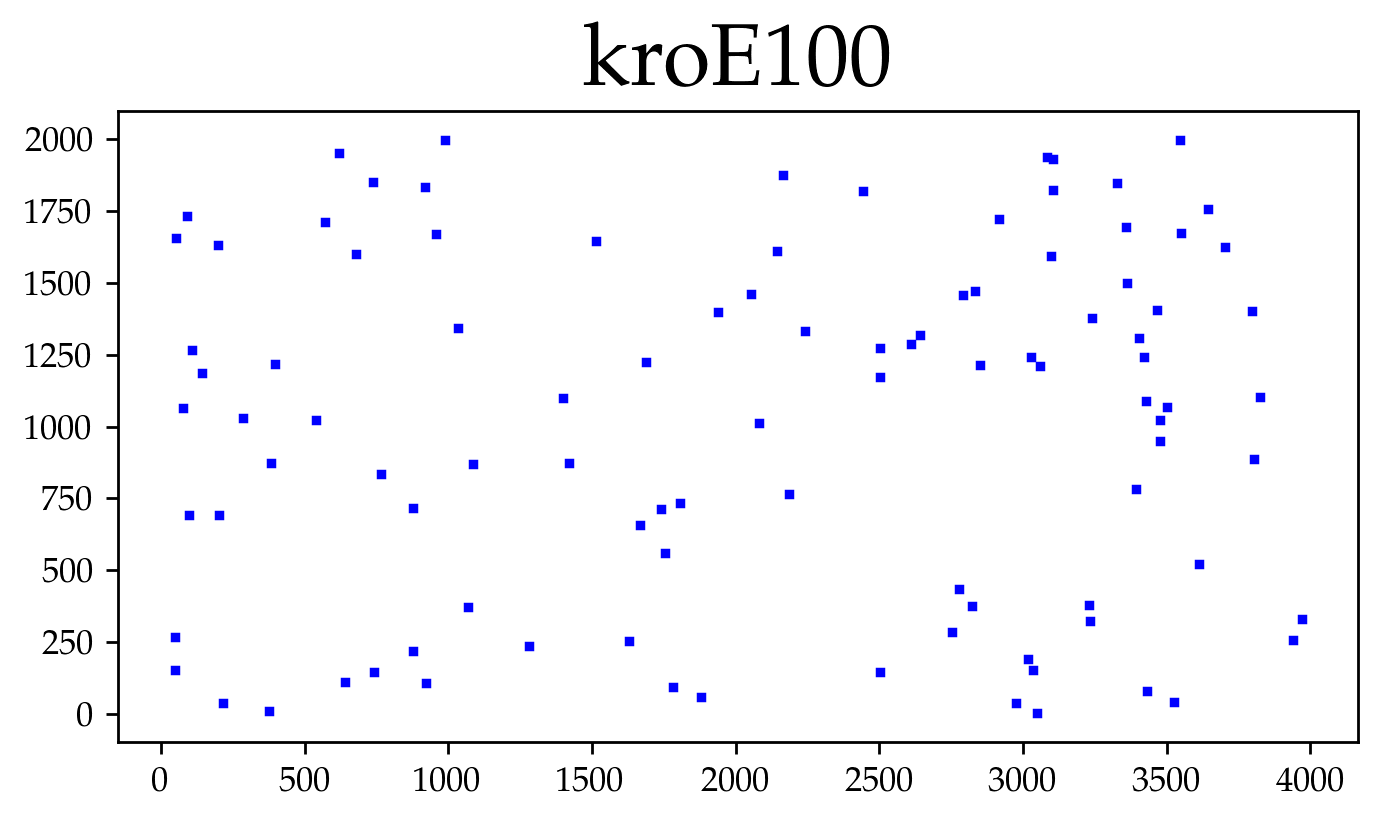
\includegraphics[width=5cm]{../tsplib_euc2d_pictures_of_instances/kroE100.png}

\end{figure}

\begin{figure}[H]
\centering
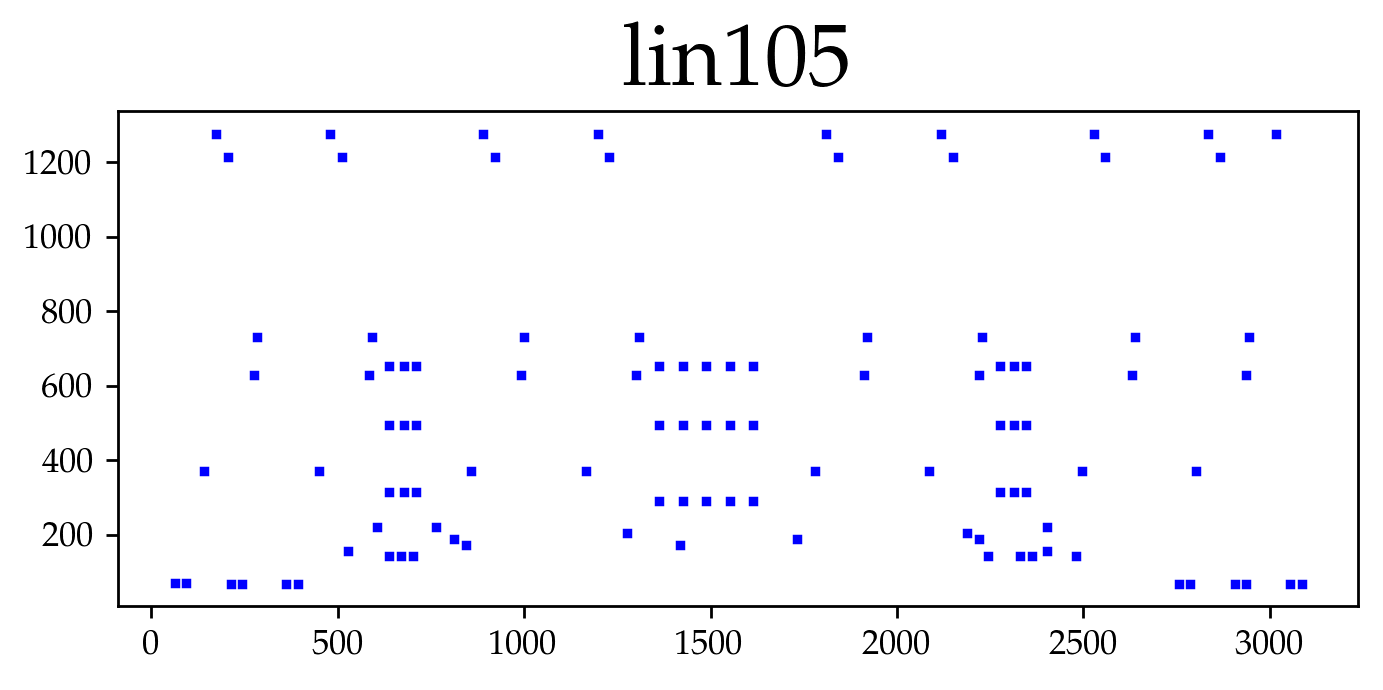
\includegraphics[width=5cm]{../tsplib_euc2d_pictures_of_instances/lin105.png}
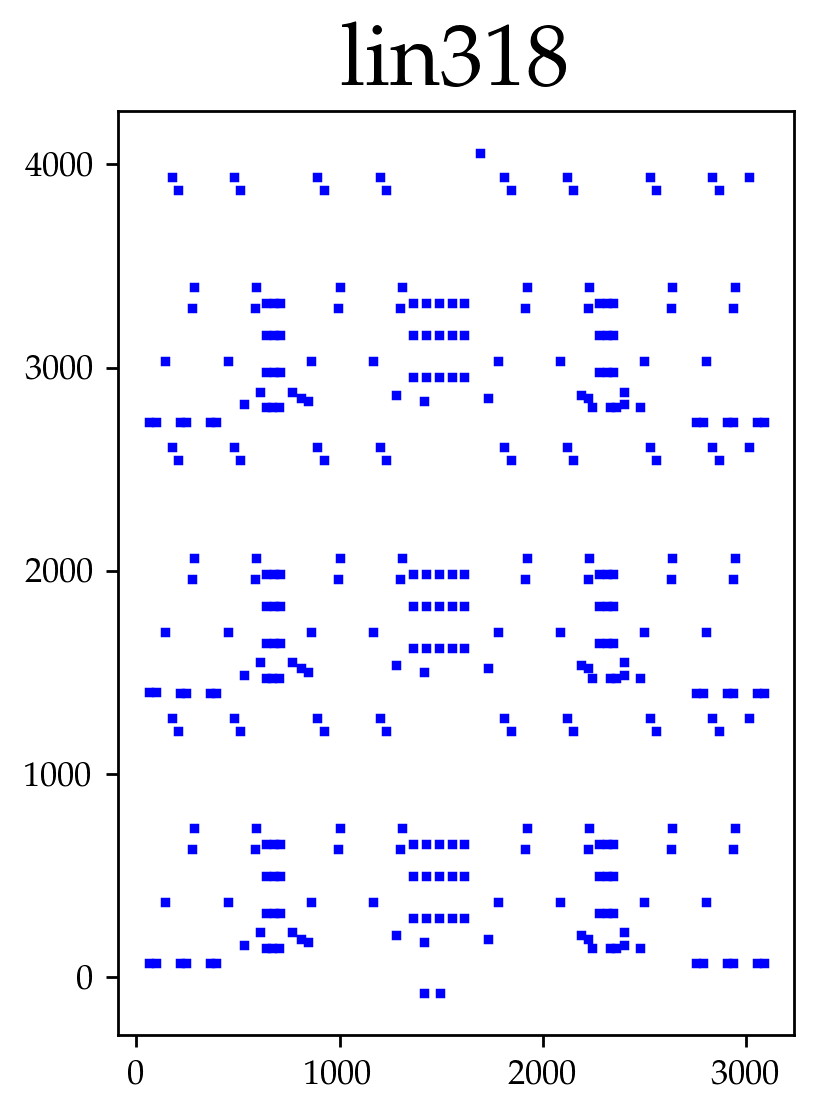
\includegraphics[width=5cm]{../tsplib_euc2d_pictures_of_instances/lin318.png}
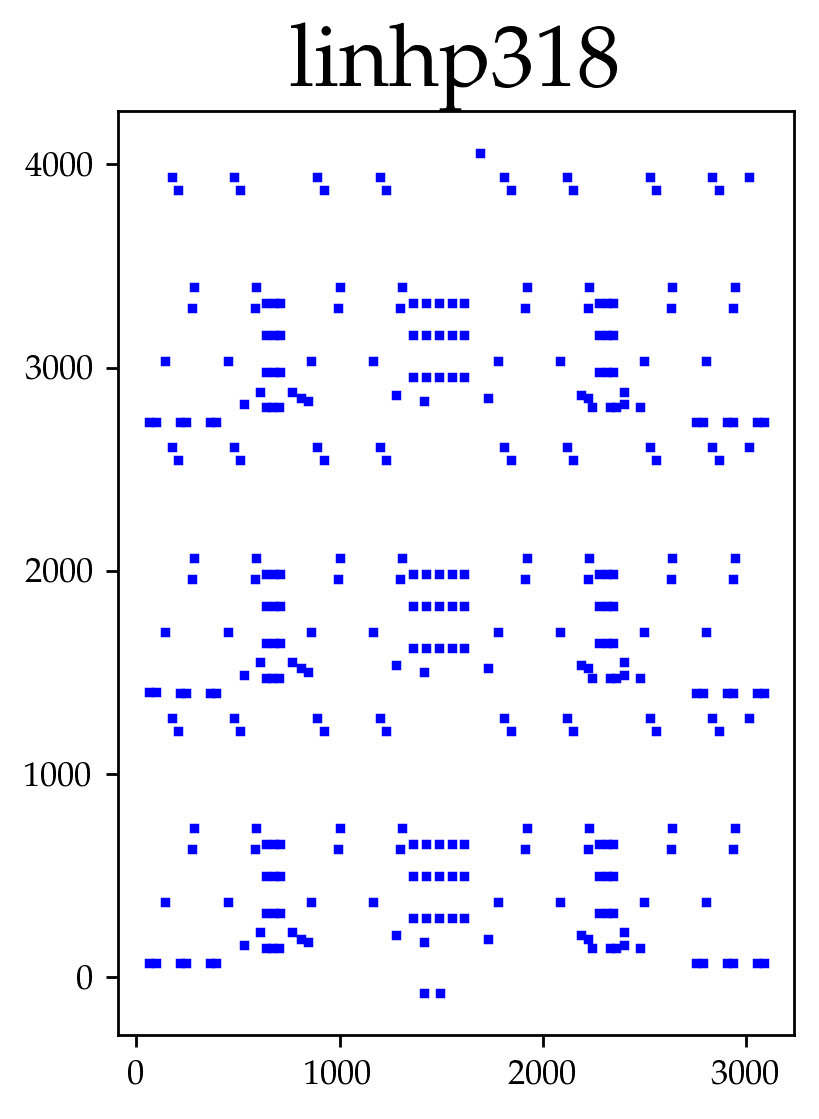
\includegraphics[width=5cm]{../tsplib_euc2d_pictures_of_instances/linhp318.png}
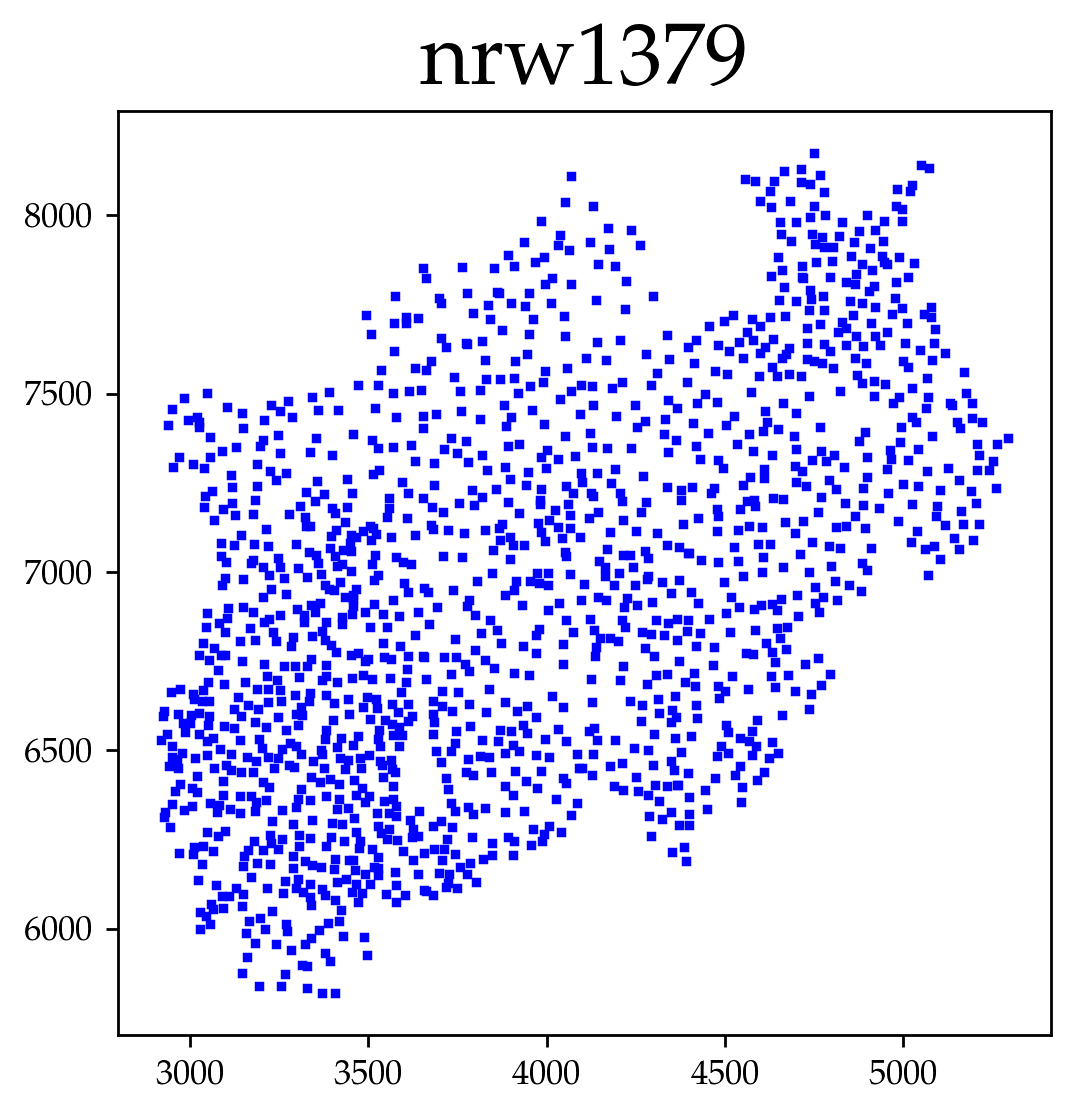
\includegraphics[width=5cm]{../tsplib_euc2d_pictures_of_instances/nrw1379.png}
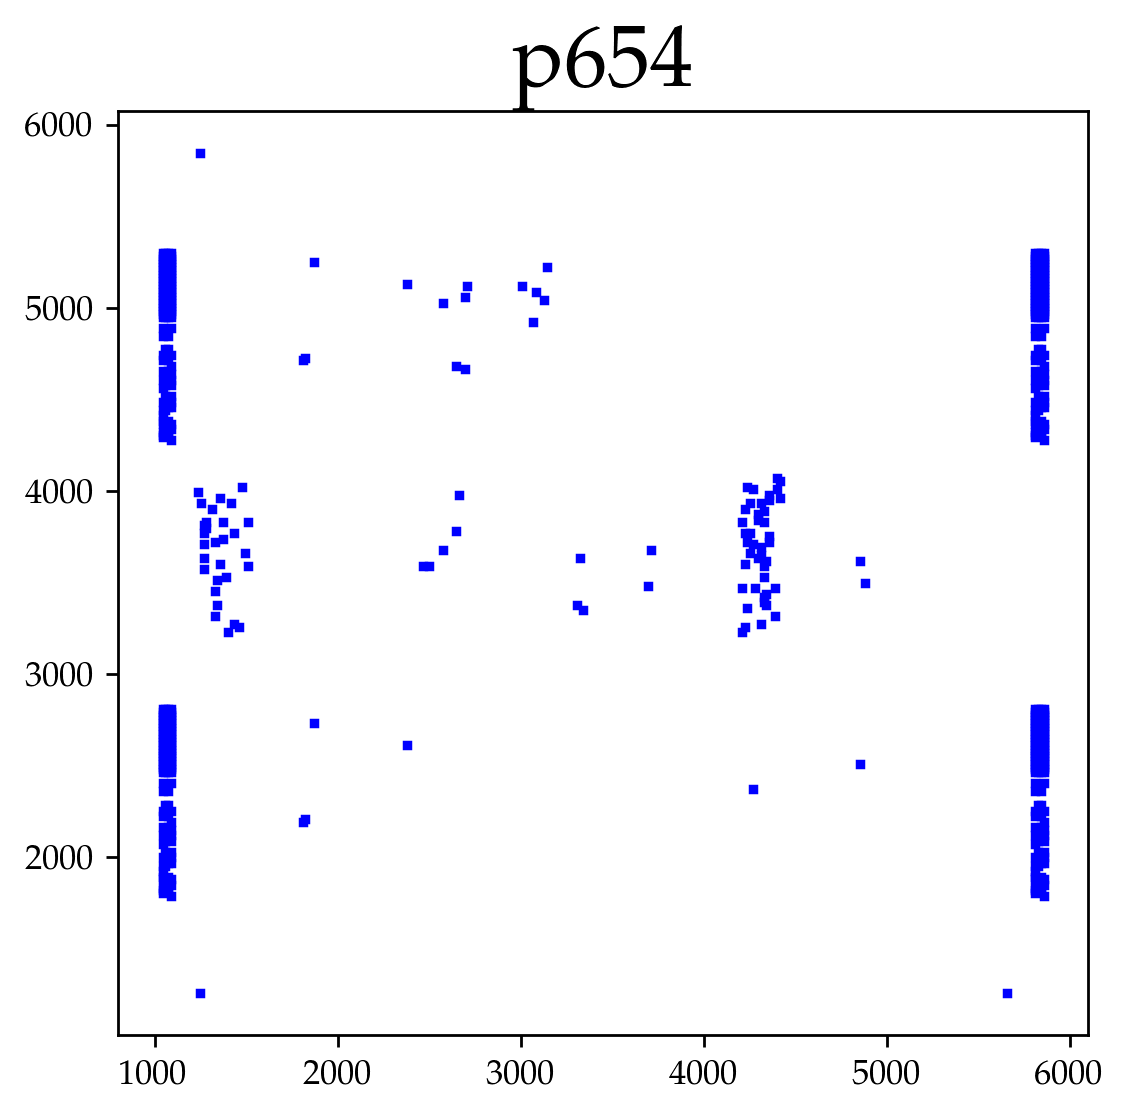
\includegraphics[width=5cm]{../tsplib_euc2d_pictures_of_instances/p654.png}
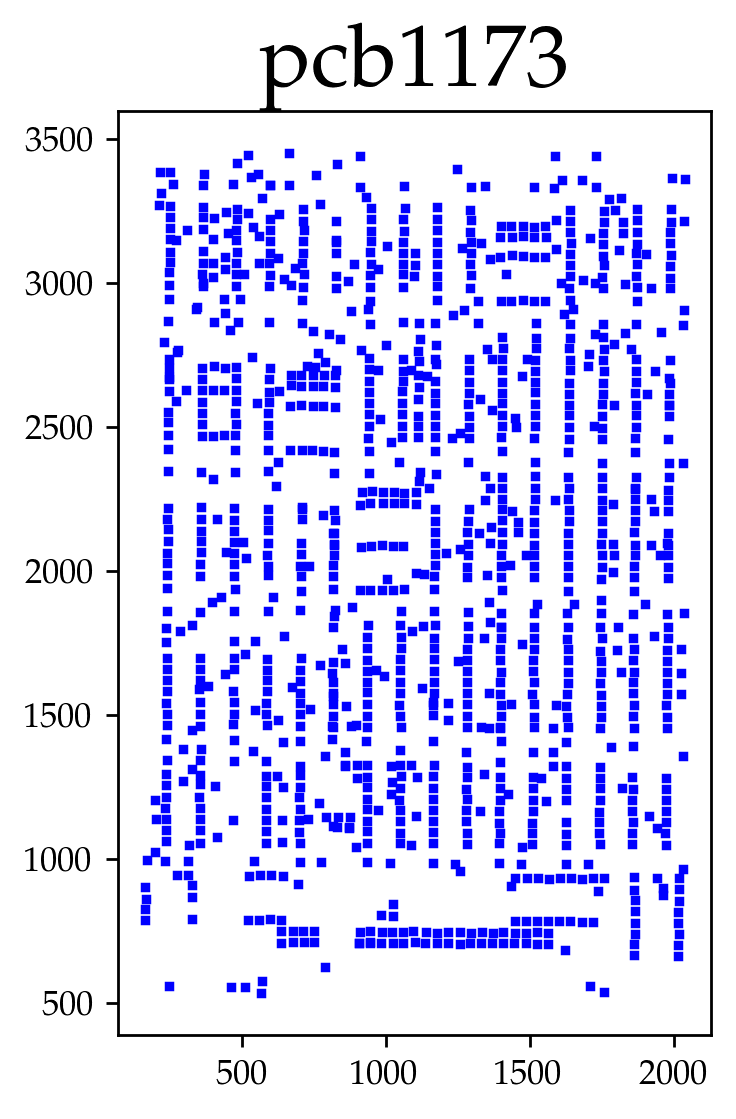
\includegraphics[width=5cm]{../tsplib_euc2d_pictures_of_instances/pcb1173.png}

\end{figure}

\begin{figure}[H]
\centering
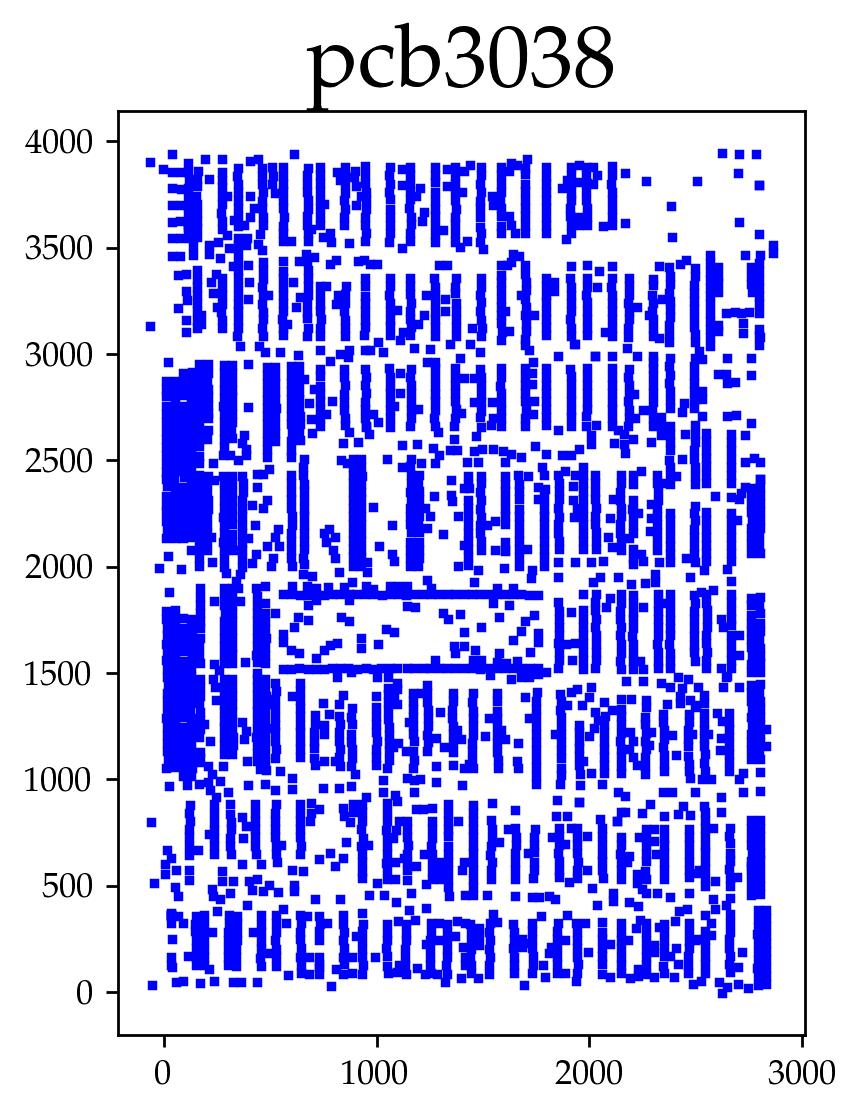
\includegraphics[width=5cm]{../tsplib_euc2d_pictures_of_instances/pcb3038.png}
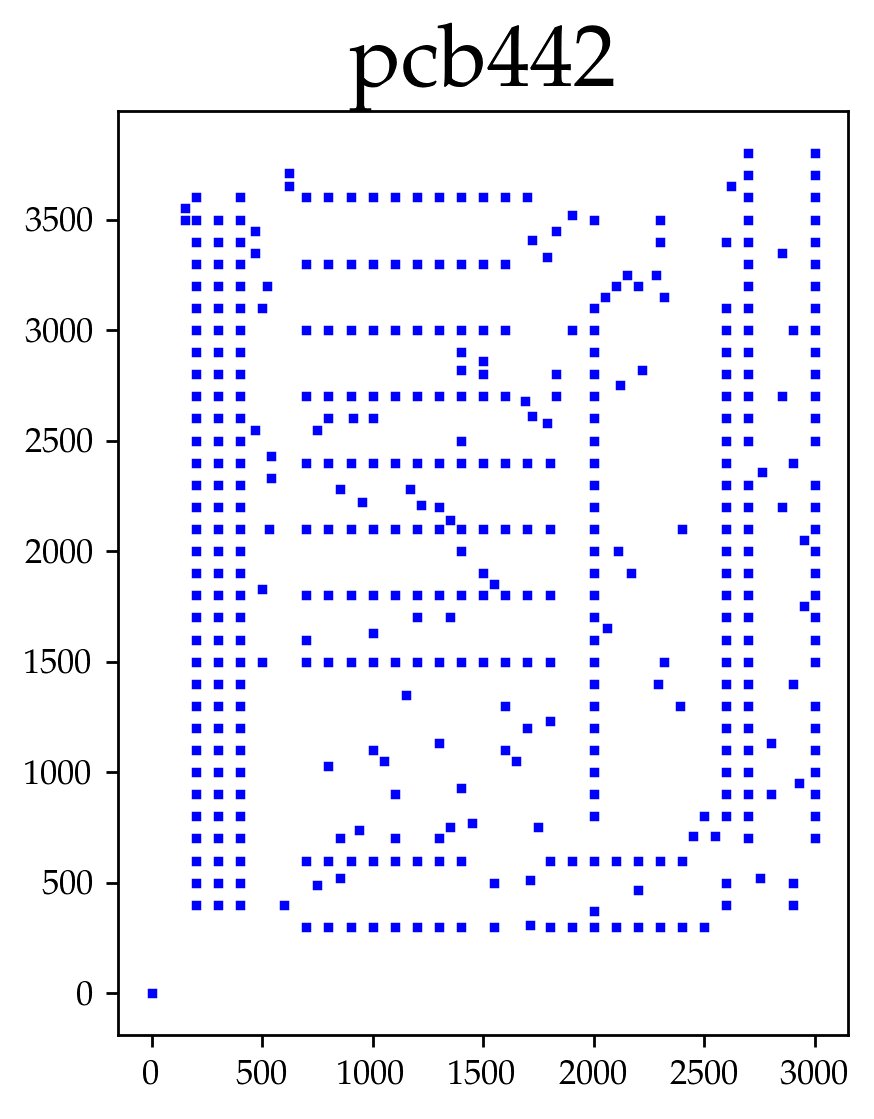
\includegraphics[width=5cm]{../tsplib_euc2d_pictures_of_instances/pcb442.png}
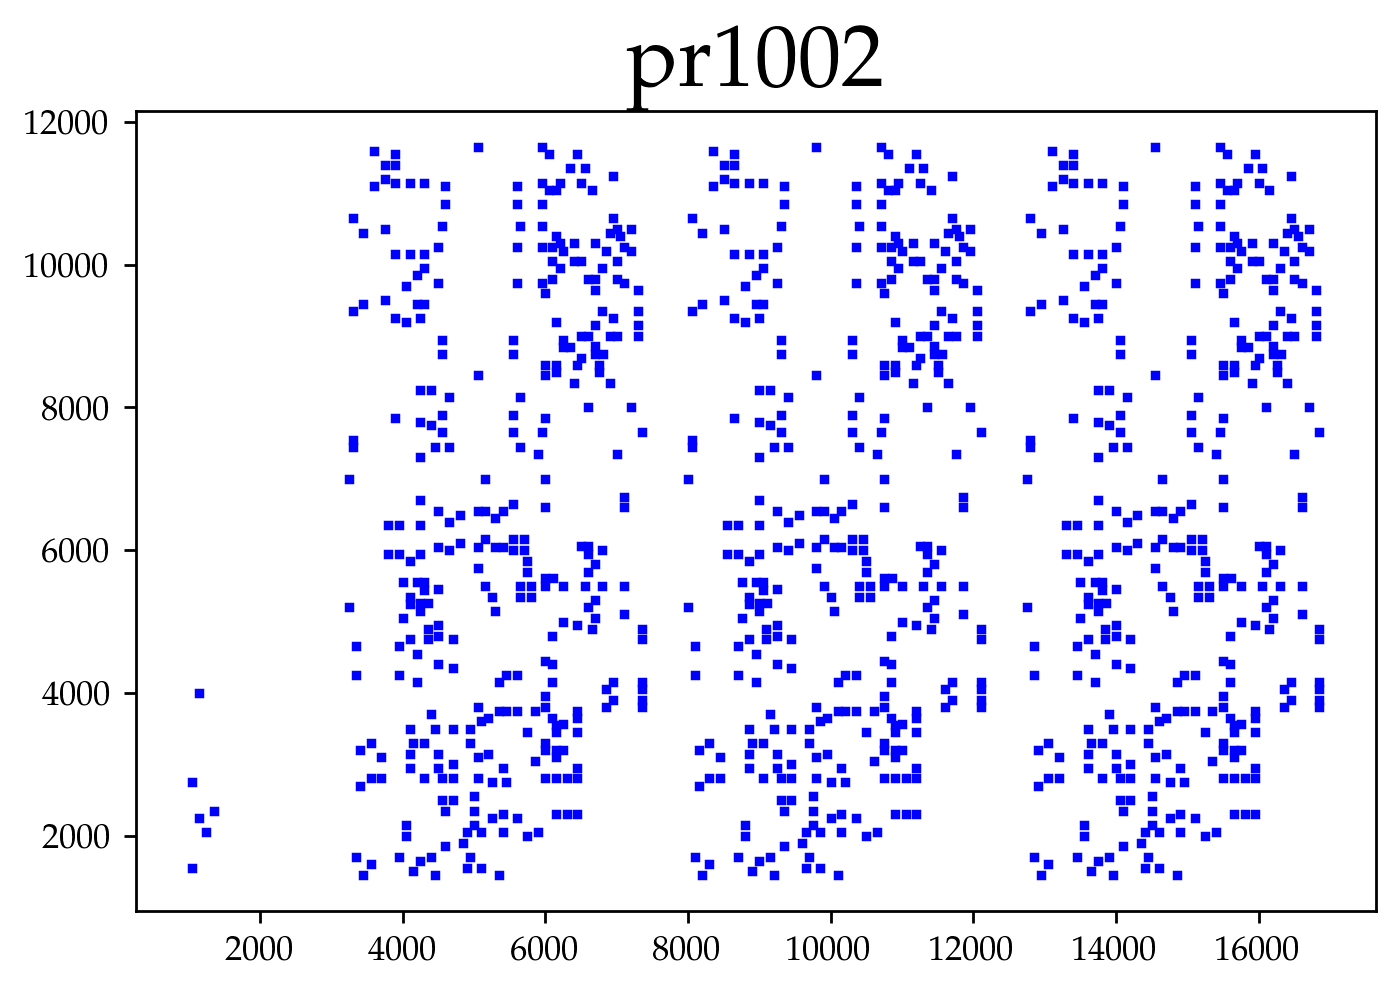
\includegraphics[width=5cm]{../tsplib_euc2d_pictures_of_instances/pr1002.png}
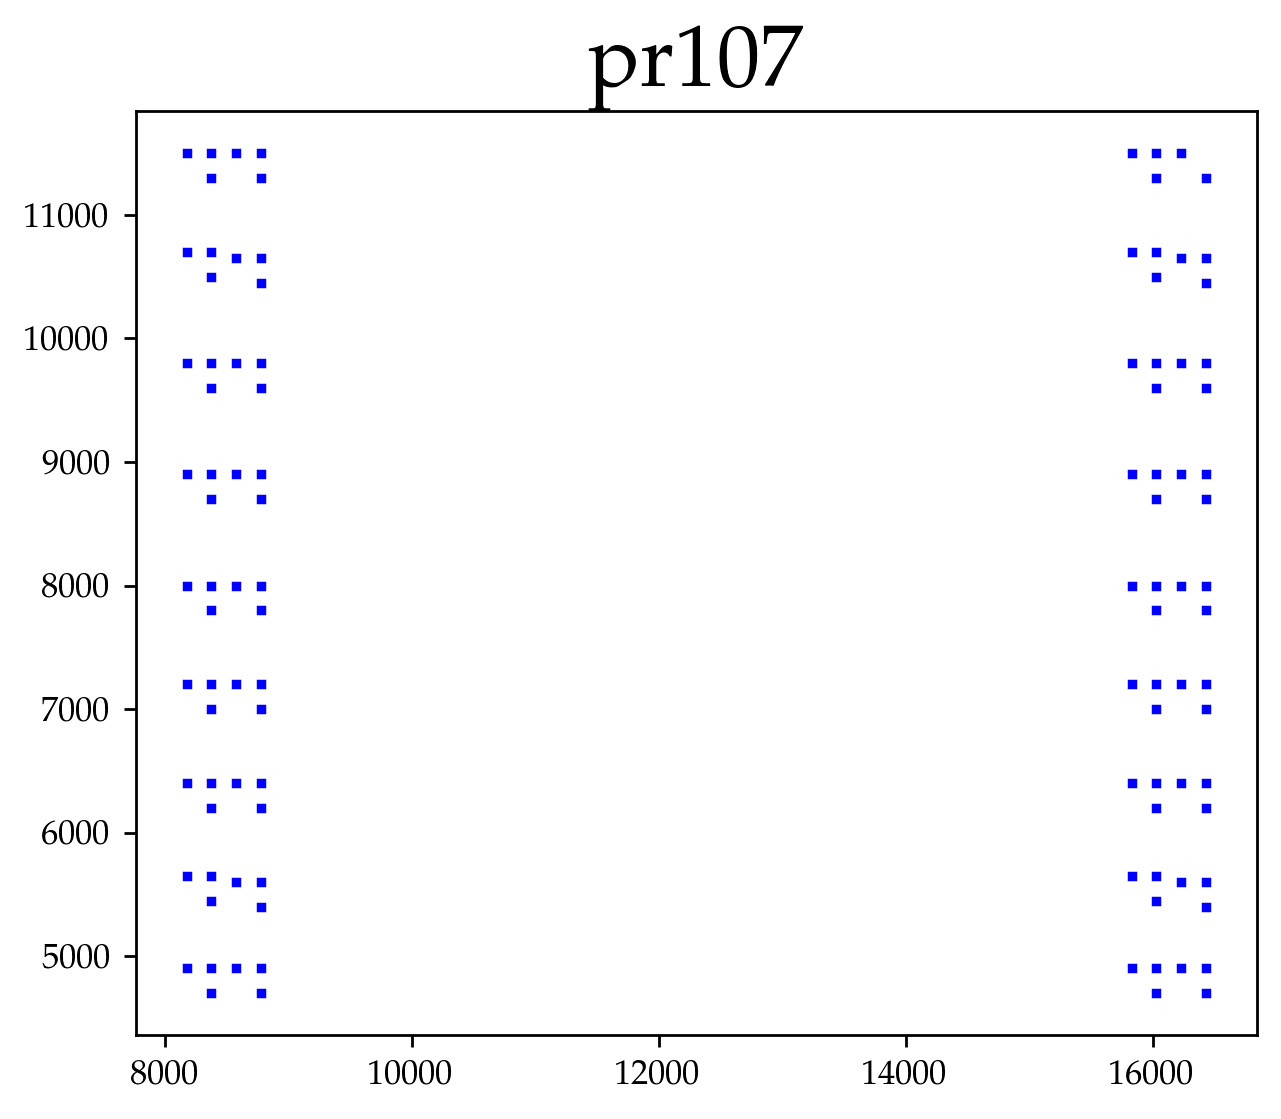
\includegraphics[width=5cm]{../tsplib_euc2d_pictures_of_instances/pr107.png}
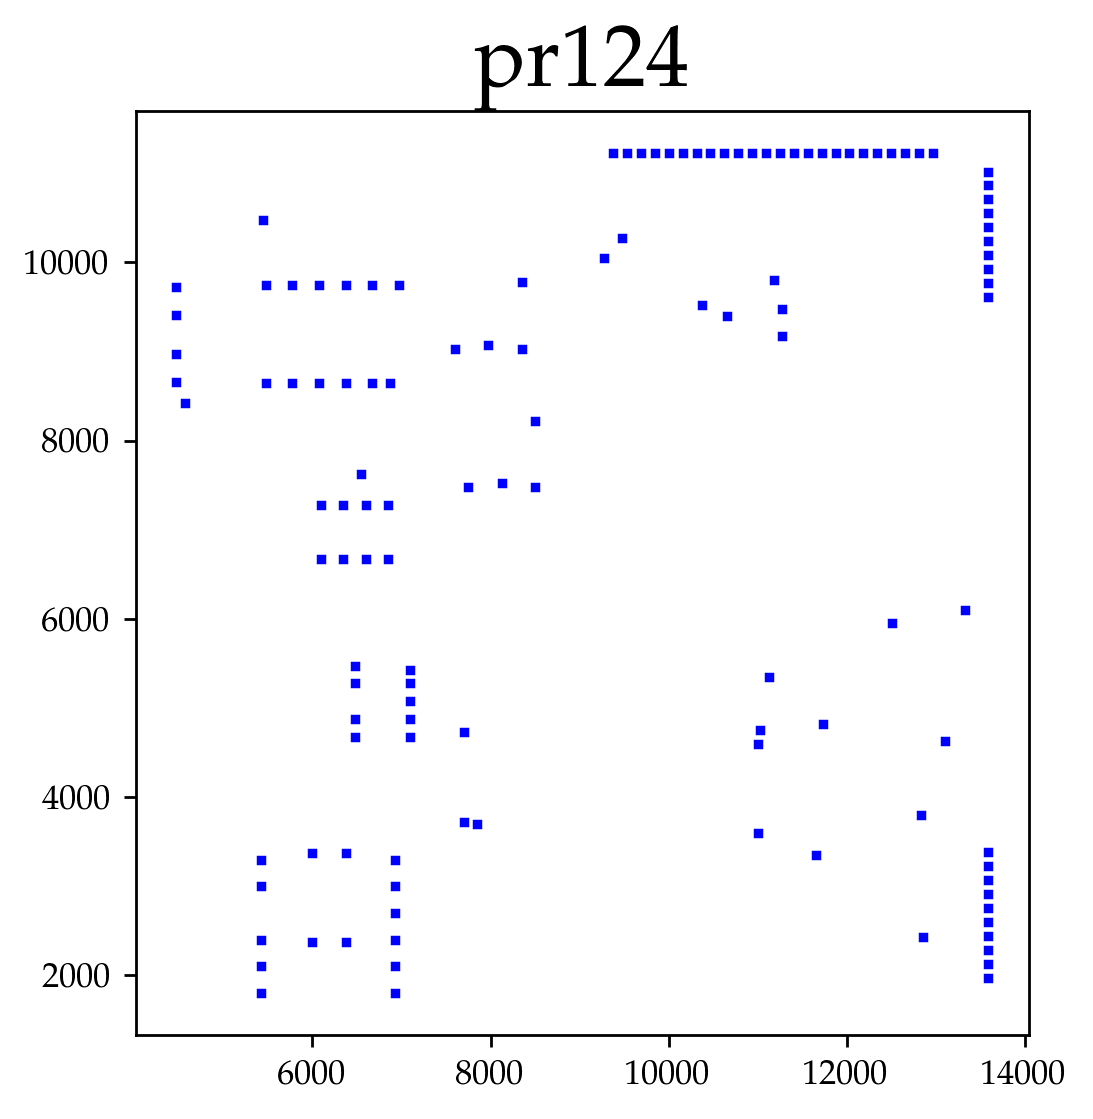
\includegraphics[width=5cm]{../tsplib_euc2d_pictures_of_instances/pr124.png}
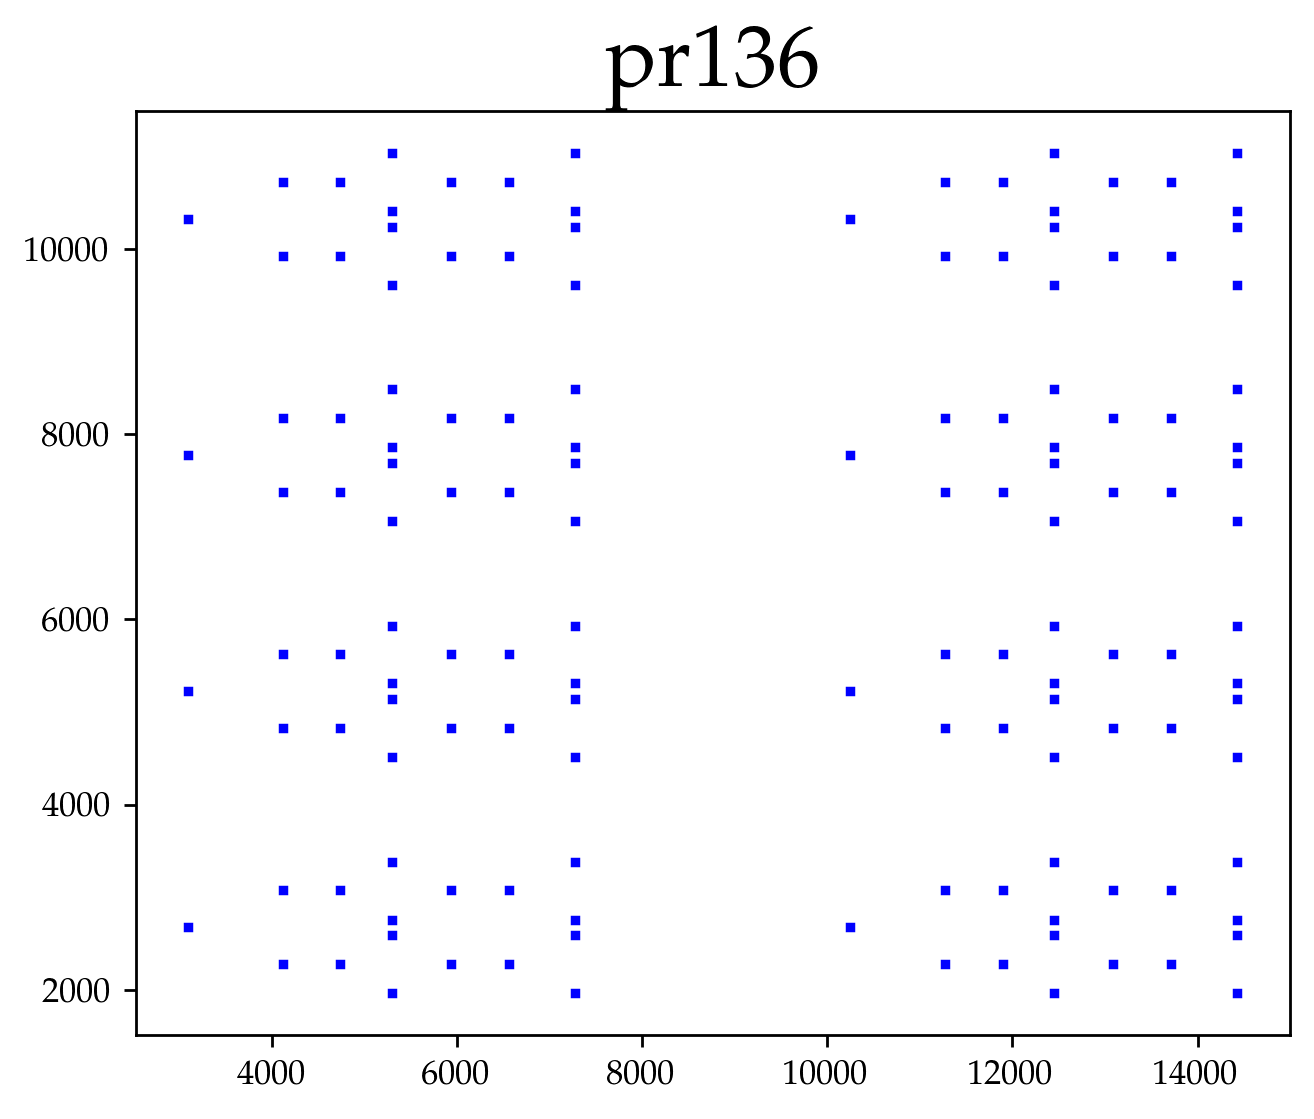
\includegraphics[width=5cm]{../tsplib_euc2d_pictures_of_instances/pr136.png}
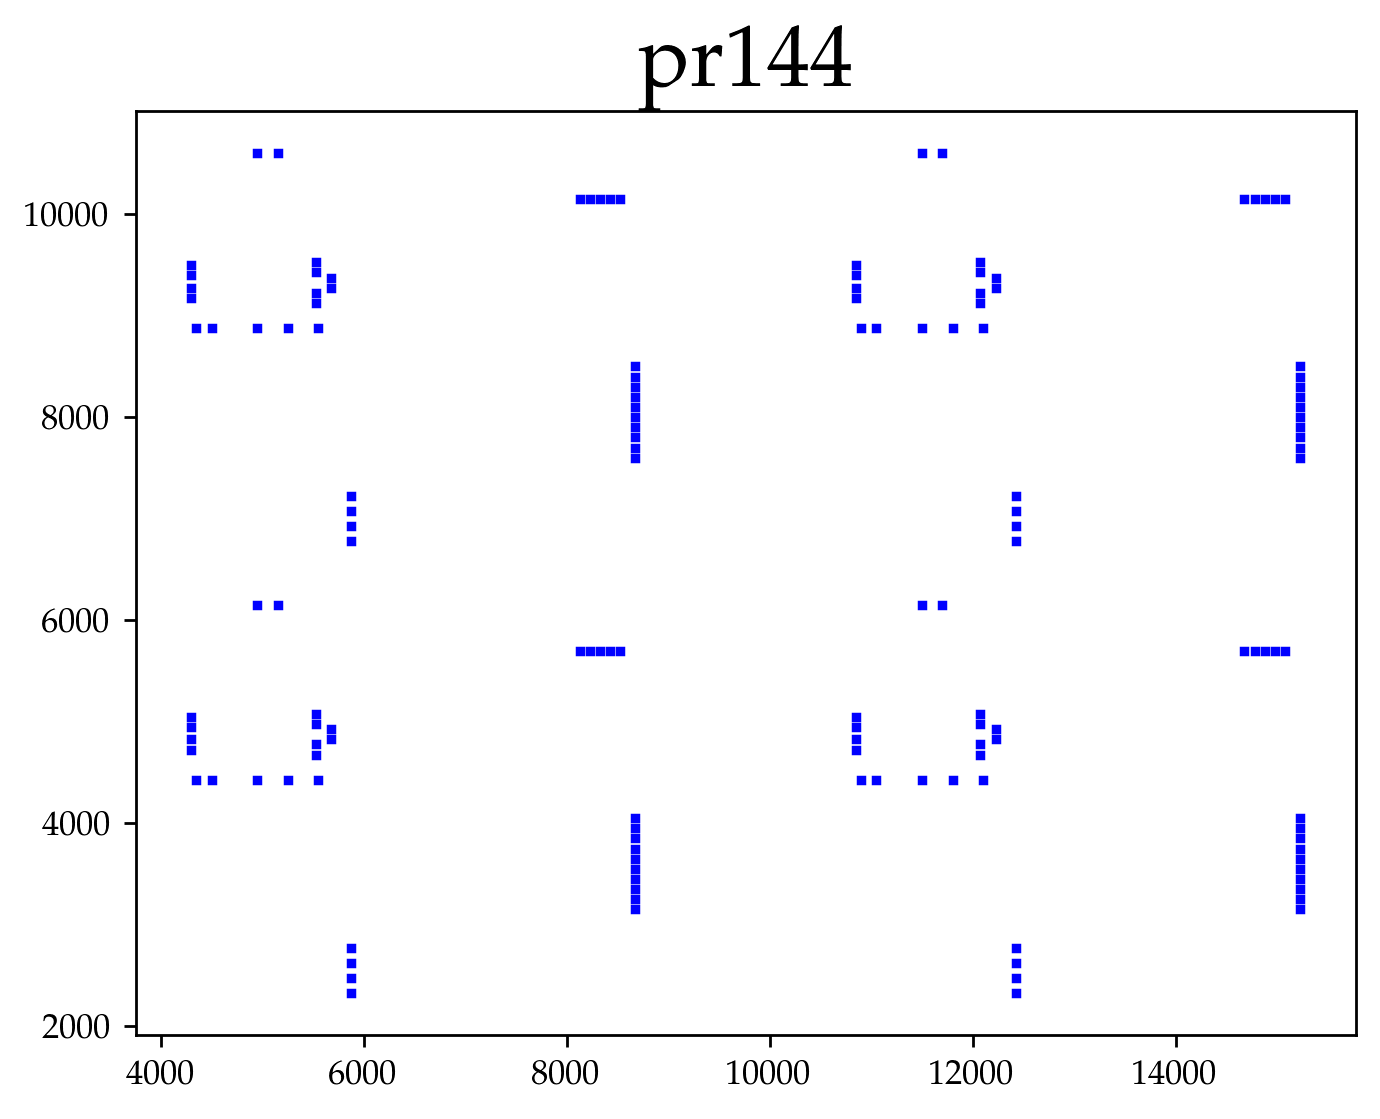
\includegraphics[width=5cm]{../tsplib_euc2d_pictures_of_instances/pr144.png}

\end{figure}

\begin{figure}[H]
\centering
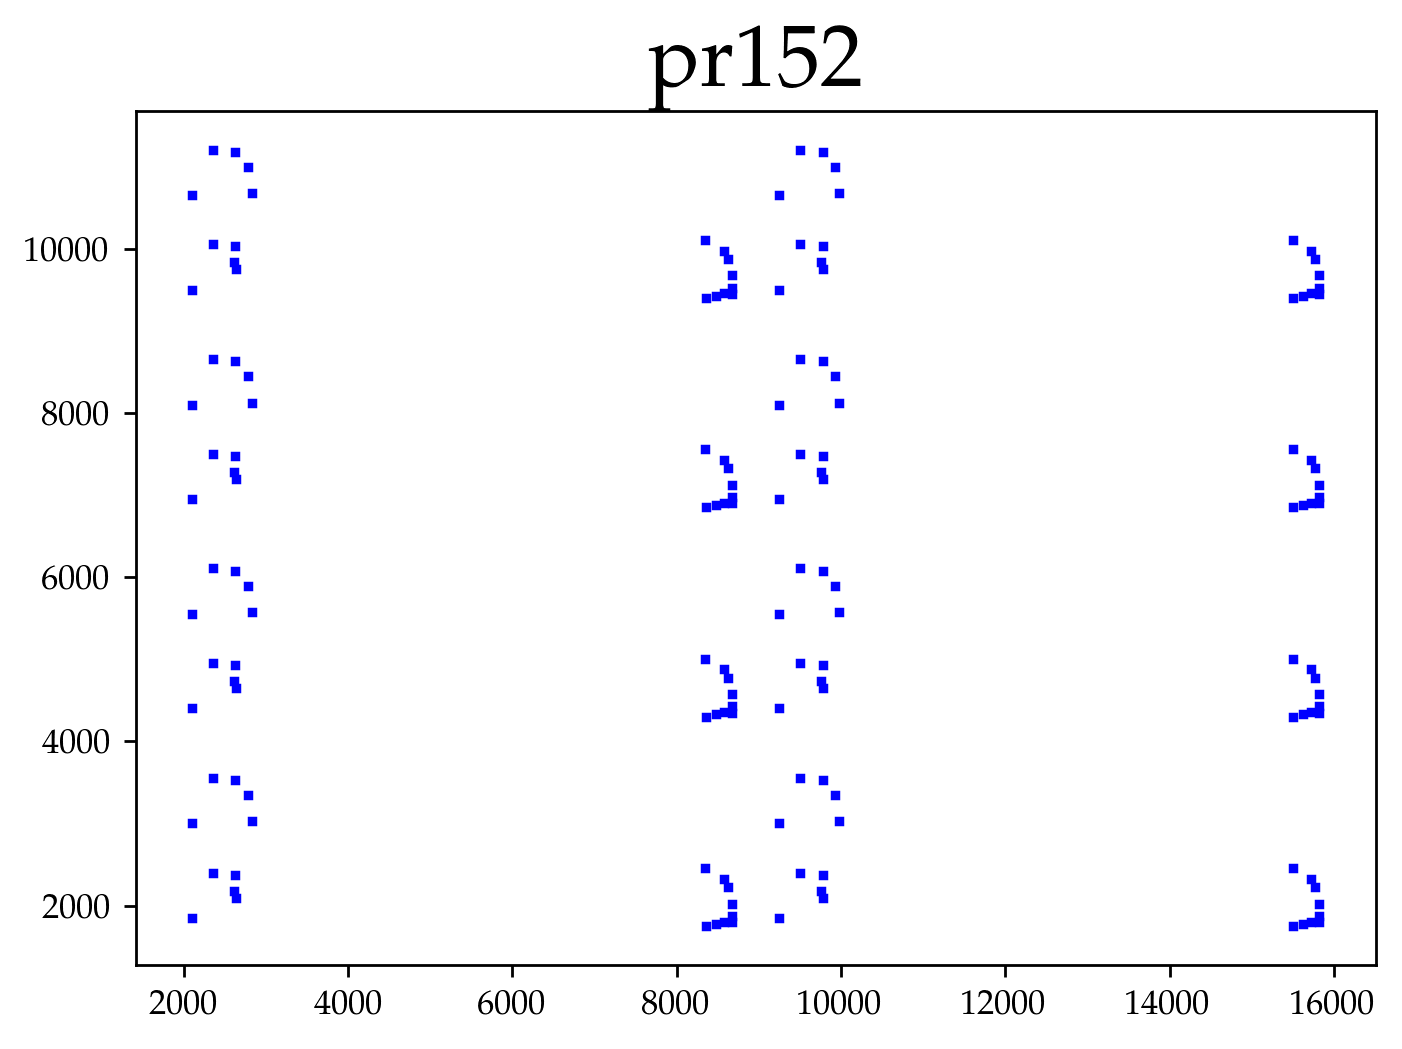
\includegraphics[width=5cm]{../tsplib_euc2d_pictures_of_instances/pr152.png}
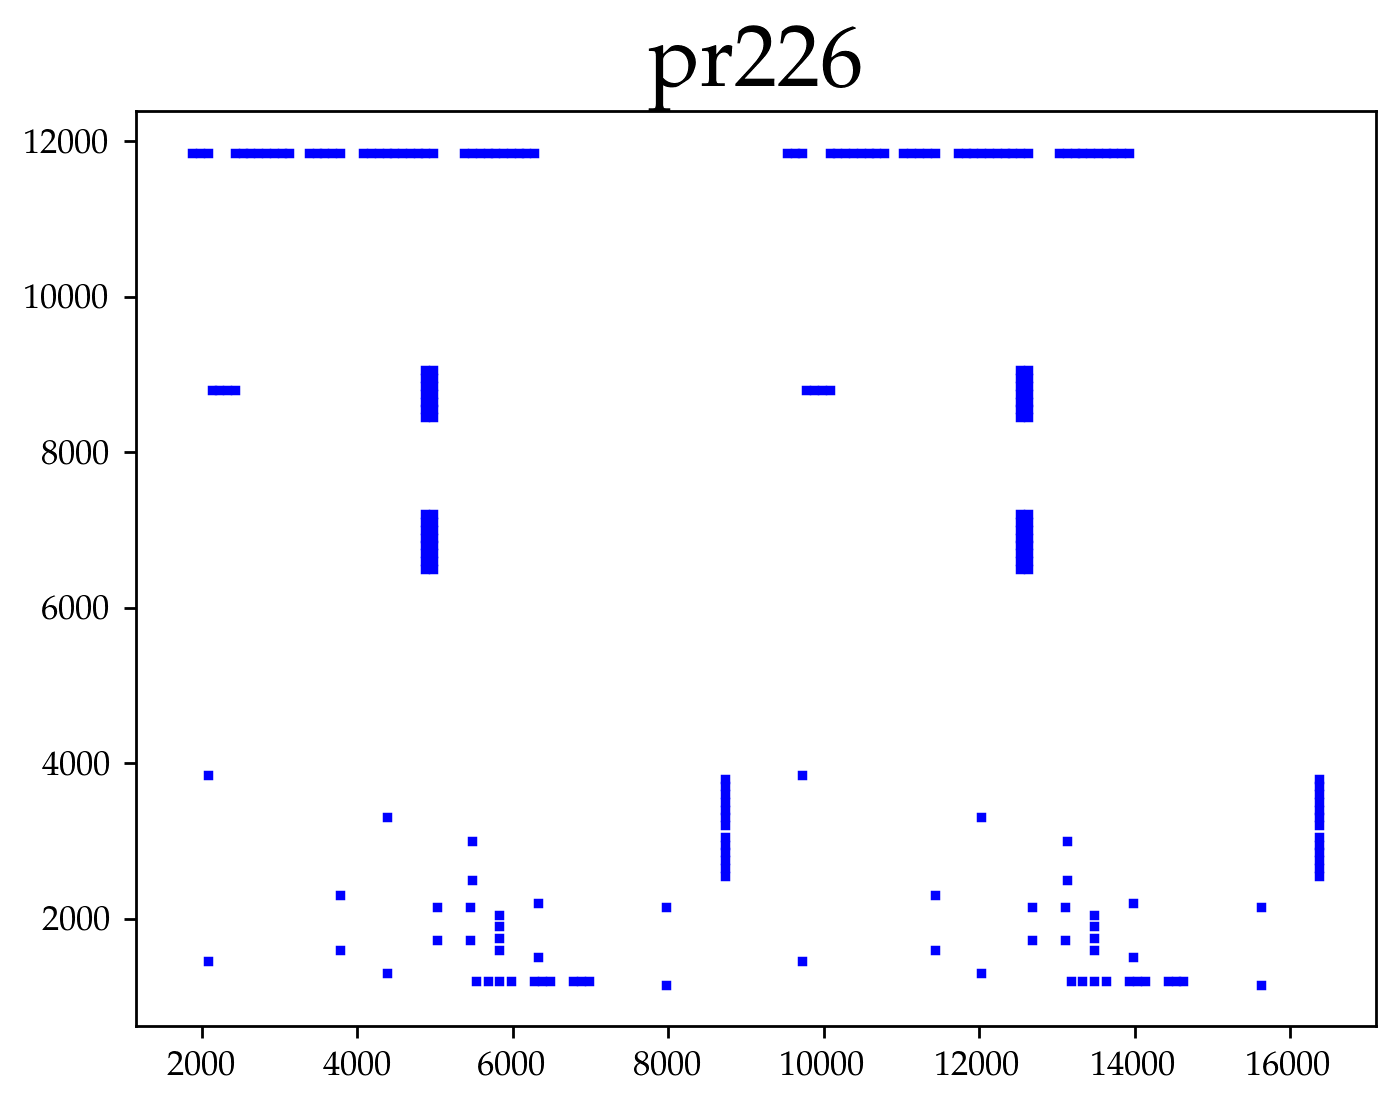
\includegraphics[width=5cm]{../tsplib_euc2d_pictures_of_instances/pr226.png}
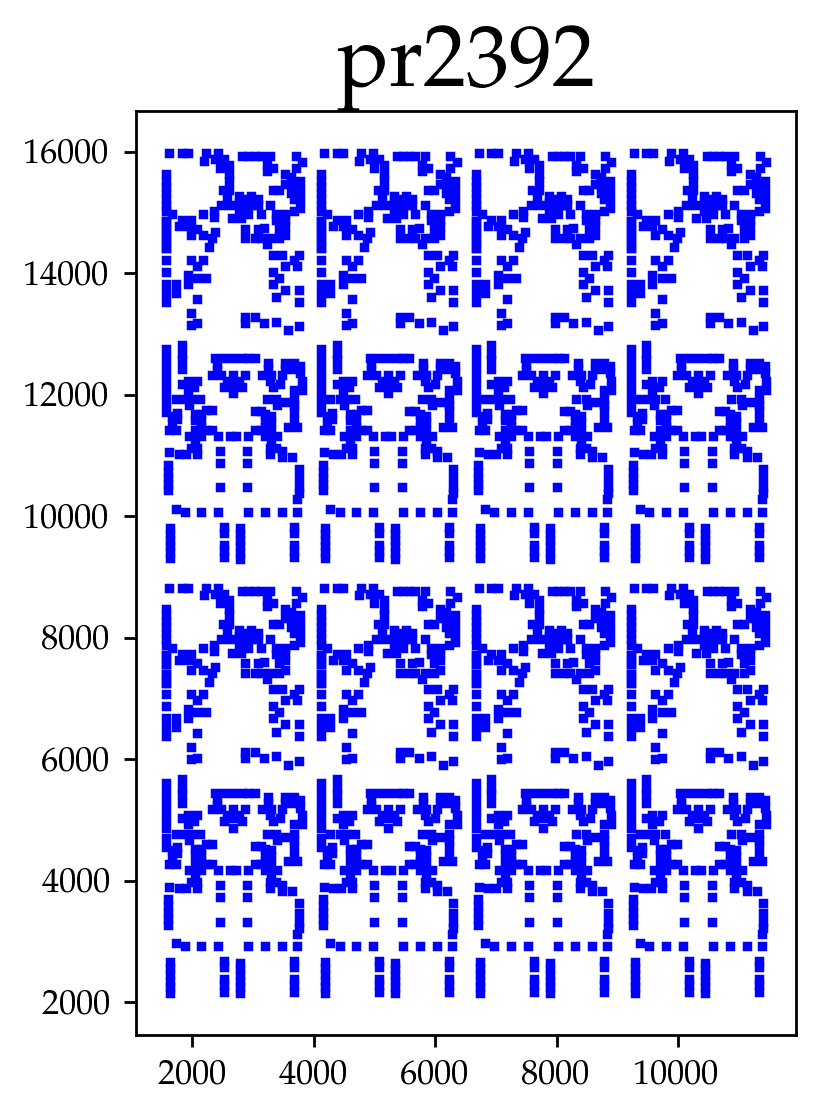
\includegraphics[width=5cm]{../tsplib_euc2d_pictures_of_instances/pr2392.png}
\includegraphics[width=5cm]{../tsplib_euc2d_pictures_of_instances/pr264.png}
\includegraphics[width=5cm]{../tsplib_euc2d_pictures_of_instances/pr299.png}

\end{figure}

\begin{figure}[H]
\centering
\includegraphics[width=5cm]{../tsplib_euc2d_pictures_of_instances/pr439.png}
\includegraphics[width=5cm]{../tsplib_euc2d_pictures_of_instances/pr76.png}
\includegraphics[width=5cm]{../tsplib_euc2d_pictures_of_instances/rat195.png}
\includegraphics[width=5cm]{../tsplib_euc2d_pictures_of_instances/rat575.png}
\includegraphics[width=5cm]{../tsplib_euc2d_pictures_of_instances/rat783.png}
\includegraphics[width=5cm]{../tsplib_euc2d_pictures_of_instances/rat99.png}

\end{figure}

\begin{figure}[htbp]
\centering
\includegraphics[width=5cm]{../tsplib_euc2d_pictures_of_instances/rd100.png}
\includegraphics[width=5cm]{../tsplib_euc2d_pictures_of_instances/rd400.png}
\includegraphics[width=5cm]{../tsplib_euc2d_pictures_of_instances/rl11849.png}
\includegraphics[width=5cm]{../tsplib_euc2d_pictures_of_instances/rl1304.png}
\includegraphics[width=5cm]{../tsplib_euc2d_pictures_of_instances/rl1323.png}
\includegraphics[width=5cm]{../tsplib_euc2d_pictures_of_instances/rl1889.png}
\includegraphics[width=5cm]{../tsplib_euc2d_pictures_of_instances/rl5915.png}
\includegraphics[width=5cm]{../tsplib_euc2d_pictures_of_instances/rl5934.png}

\end{figure}

\begin{figure}[H]
\centering
\includegraphics[width=5cm]{../tsplib_euc2d_pictures_of_instances/st70.png}
\includegraphics[width=5cm]{../tsplib_euc2d_pictures_of_instances/ts225.png}
\includegraphics[width=5cm]{../tsplib_euc2d_pictures_of_instances/tsp225.png}
\includegraphics[width=5cm]{../tsplib_euc2d_pictures_of_instances/u1060.png}
\includegraphics[width=5cm]{../tsplib_euc2d_pictures_of_instances/u1432.png}
\includegraphics[width=5cm]{../tsplib_euc2d_pictures_of_instances/u159.png}
\includegraphics[width=5cm]{../tsplib_euc2d_pictures_of_instances/u1817.png}

\end{figure}

\begin{figure}[H]
\centering
\includegraphics[width=5cm]{../tsplib_euc2d_pictures_of_instances/u2152.png}
\includegraphics[width=5cm]{../tsplib_euc2d_pictures_of_instances/u2319.png}
\includegraphics[width=5cm]{../tsplib_euc2d_pictures_of_instances/u574.png}
\includegraphics[width=5cm]{../tsplib_euc2d_pictures_of_instances/u724.png}
\includegraphics[width=5cm]{../tsplib_euc2d_pictures_of_instances/usa13509.png}
\includegraphics[width=5cm]{../tsplib_euc2d_pictures_of_instances/vm1084.png}
\includegraphics[width=5cm]{../tsplib_euc2d_pictures_of_instances/vm1748.png}
 \end{figure}


%\input{laundry-list-questions.tex}



\newpage
\section{Machine Details}

The code is being developed on a laptop, with the following specs:

\definecolor{graylt}{rgb}{0.75, 0.75, 0.75}
\footnotesize
\texttt{
\begin{center}
 \begin{tabular}{r!{\color{graylt}\vrule}l}
   Operating System &   Linux Mint 18.3 Cinnamon 64-bit \\
   Cinnamon Version &   3.6.6                           \\
   Linux Kernel     &   1.10.0-38-generic               \\
   Processor        &   Intel{\tiny\textcopyright} Core$^{\text{TM}}$ i5-4300U CPU @ 1.90 GHz x 2 \\
   Memory           &   7.5 GiB                         \\
   Hard Drives      &   109.0 GB                        \\
   Graphics Card    &   Intel Corporation Haswell-ULT Integrated Graphics Controller
  \end{tabular}
\end{center}}
\normalsize     
 
The Anaconda distribution on the machine has the following configuration: (output of `\texttt{conda info}')


\footnotesize
\texttt{
\begin{center}
 \begin{tabular}{r!{\color{graylt}\vrule}l}
      \arrayrulecolor{graylt}
          active environment & None \\  
       user config file & /home/xxxx/.condarc \\ 
 populated config files &  \\ 
          conda version & 4.7.10 \\ 
    conda-build version & 3.18.8 \\ 
         python version & 3.7.3.final.0 \\ 
       virtual packages &  \\ 
       base environment & /home/xxxx/anaconda3  (read only) \\ \hline
           channel URLs & \pbox{20cm}{\url{https://repo.anaconda.com/pkgs/main/linux-64} \\ \url{https://repo.anaconda.com/pkgs/main/noarch} \\  \url{https://repo.anaconda.com/pkgs/r/linux-64} \\ \url{https://repo.anaconda.com/pkgs/r/noarch} } \\  \hline
          package cache & \pbox{20cm}{\texttt{/home/xxxx/anaconda3/pkgs} \\ \texttt{/home/xxxx/.conda/pkgs} } \\ \hline
       envs directories & \pbox{20cm}{\texttt{/home/xxxx/.conda/envs} \\ \texttt{/home/xxxx/anaconda3/envs}} \\ \hline
               platform & linux-64 \\  \hline
             user-agent & \pbox{20cm}{conda/4.7.10 requests/2.22.0 CPython/3.7.3 \\ Linux/4.10.0-38-generic linuxmint/18.3 glibc/2.23} \\ \hline
                UID:GID & 1000:1000 \\ 
             netrc file & None \\ 
           offline mode & False 
  \end{tabular}
\end{center}}
\normalsize 





\end{appendices}
\nwenddocs{}


